\chapter{Software Specification}
		
	\section{Functional Requirements}
			
			\noindent \textbf{Stakeholders:}
			
			\begin{packed_enum}
				
				\item Developers and Maintainers
				\item Festival-goers
				\item Festival investors and sponsors
				\item Administrator			
				\item Creator
				\item Organiser
				\item Worker
				
			\end{packed_enum}
			
			\noindent \textbf{Actors and their functional requirements:}
			
			\begin{packed_enum}
				\item  \underbar{Unregistered/Guest User(initiator) can:}
				\begin{packed_enum}
					\item Register a new account - fill in the form
					\begin{packed_enum}
						\item Username
						\item Email
						\item Password
						\item Password Verification
						\item Phone Number
						\item Name
						\item Surname
						\item Desired Role
						\begin{packed_enum}
							\item Leader
							\item Organiser
							\item Worker
						\end{packed_enum}
					\end{packed_enum}
					
					\item Log in - fill in the form
					\begin{packed_enum}
						\item Username or Email
						\item Password
					\end{packed_enum}
					
				\end{packed_enum}
				
				\item  \underbar{Administrator can:}
				\begin{packed_enum}
					\item Access the list of Users
					\item Verify Creators
					\item Moderate Users' details and/or ban them as to alleviate abuse/misuse
					
					\item Access the list of Festivals
					\begin{packed_enum}
						\item Access the list of Jobs
						\begin{packed_enum}
							\item Access the list of corresponding Activities
							\item Access the list of Workers
						\end{packed_enum}
						\item Moderate Festivals, Jobs and Activities and/or veto/delete them as to alleviate abuse/misuse
					\end{packed_enum}
					
				\end{packed_enum}
				
				\item	\underbar{Leaders manage Festivals:}
				\begin{packed_enum}
					\item Create [multiple] Festivals
					\item Modify or delete their Festivals	
					\item Inherit Organiser functionalities for their own Festivals
					\item Appoint Organisers to their Festivals(check if the selected Organiser is organising any possibly concurrent Festivals)
					\item Access the Jobs, Activities, Workers and other details of their Festival
				\end{packed_enum}
				
				\item	\underbar{Organiser organises the concrete Festival workflow:}
				\begin{packed_enum}
					\item Job management
					\begin{packed_enum}
						\item Select which Jobs need to be done - open their corresponding Job Auctions
						\item Job Sequence - order and parallelise Jobs - Festival Job Timeline
						\item Ability to extend Job Auction lifetime by 1 day
						\item View and modify Jobs
						\begin{packed_enum}
							\item Access Workers' profiles, details, comments, ...
							\item Access Job description, Time and Location - modify them as needed
							\item View each Job's list of Activities
						\end{packed_enum}
					\end{packed_enum}
					
					\item Organise a Festival -- Ability to organise multiple Festivals - check for concurrency!
				\end{packed_enum}
				
				\item \underbar {Workers perform specific Jobs. They can:}
				\begin{packed_enum}
					\item Select their fields of specialisation
					\item Apply to Job Auctions
					\item Perform Job - can perform multiple Jobs - check for concurrency
					\item Fill out Job information sheet
					\begin{packed_enum}
						\item Job Description
						\item Job Location and Time
						\item Form a list of Activities that need to be done - ability to modify, add and/or delete the entries in this list
					\end{packed_enum}
				\end{packed_enum}
				
			\end{packed_enum}
			\eject
				
			\subsection{Use Cases}
				
				\subsubsection{Use Cases Description}
					
				\noindent \underbar{\textbf{UC2 - Registration}}
				\begin{packed_item}
					\item \textbf{Main Stakeholders:} Unregistered/Guest Users
					\item \textbf{Goal:} Register a new User Account
					\item \textbf{Stakeholders:} Database
					\item \textbf{Conditions:} Must not be logged in, and must be located at the Login screen.
					\item \textbf{Event flow description: }
					\begin{packed_enum}
						\item The User is located at the login screen, and taps the 'Create one' button, located next to the 'No account yet?' label
						\item A new Screen pops up - Guest fills the Registration Form
						\item Upon tapping 'Create Account' a new account is created and stored in the Database
					\end{packed_enum}
				
					\begin{packed_item}
						\item[2.a] Illegal input
						\item[] \begin{packed_enum}
							\item An error message is displayed informing the User that they have entered illegal input
							\item The notification asks the User to re-format and re-enter the input. The expected format and rules are displayed
							\item The steps above are repeated if new input isn't accepted either
						\end{packed_enum}
						
						\item[3.a] Data not successfully sent and parsed on the Server
						\item[] \begin{packed_enum}
							\item An error message is displayed informing the User that an error has occurred
							\item A 'Retry' button is displayed on the screen - upon clicking it the form is resent and parsing tried again
							\item The User is notified upon success
						\end{packed_enum}
						
					\end{packed_item}
					
				\end{packed_item}
			
				\noindent \underbar{\textbf{UC3 - Log-In}}
				\begin{packed_item}
					\item \textbf{Main Stakeholders:} Guest Users who have a registered account
					\item \textbf{Goal:} Log into the platform
					\item \textbf{Stakeholders:} Database
					\item \textbf{Conditions:} Must not be logged in, and must be located at the Login screen.
					\item \textbf{Event flow description: }
					\begin{packed_enum}
						\item User enter the email or username and their password
						\item User taps the `Log-in` button
						\item Database checks the data and if login is successful the user is logged in
					\end{packed_enum}
				
					\begin{packed_item}
						\item[3.a] Email/Username and Password combination is wrong and the User isn't logged in.
						\item[] \begin{packed_enum}
							\item The fields Email/Username and Password are reset
							\item An error message is displayed
							\item User needs to enter the log-in data again
						\end{packed_enum}
					
						\item[3.a] Data not successfully sent and parsed on the Server
						\item[] \begin{packed_enum}
							\item An error message is displayed informing the User that an error has occurred
							\item A 'Retry' button is displayed on the screen - upon clicking it the form is resent and parsing tried again
							\item The User is notified upon success
						\end{packed_enum}
					\end{packed_item}
				\end{packed_item}
			
				\noindent \underbar{\textbf{UC4 - Account Data Overview}}
				\begin{packed_item}
					\item \textbf{Main Stakeholders:} User
					\item \textbf{Goal:} View the account data
					\item \textbf{Stakeholders:} Database
					\item \textbf{Conditions:} Must be logged in
					\item \textbf{Event flow description: }
					\begin{packed_enum}
						\item User taps the corresponding button, and views his profile information
						\item Data is retrieved from the Database
						\item A screen depicting Account data appears
					\end{packed_enum}
					
					\begin{packed_item}
						\item[2.a] Data not successfully retrieved
						\item[] \begin{packed_enum}
							\item An error message is displayed informing the User data couldn't be retrieved
							\item A 'Retry' button is displayed on the screen - upon clicking it the app attempts to fetch data again
							\item Upon successful data retrieval(If ever) the button and error message are removed and then the data is displayed
						\end{packed_enum}
					\end{packed_item}
				\end{packed_item}
			
				\noindent \underbar{\textbf{UC7 - Verifying a Leader}}
				\begin{packed_item}
					\item \textbf{Main Stakeholders:} Administrators
					\item \textbf{Goal:} Check, and if all is in order, verify a Leader
					\item \textbf{Stakeholders:} Database, Leader
					\item \textbf{Conditions:} Must be logged in. There is a Leader awaiting confirmation.
					\item \textbf{Event flow description: }
					\begin{packed_enum}
						\item The list of Leaders is displayed to the Administrator
						\item Data is fetched from the Database
						\item Administrator decides whether to verify or deny the Leader
					\end{packed_enum}
					
					\begin{packed_item}
						\item[2.a] Data not successfully retrieved
						\item[] \begin{packed_enum}
							\item An error message is displayed informing the User data couldn't be retrieved
							\item A 'Retry' button is displayed on the screen - upon clicking it the app attempts to fetch data again
							\item Upon successful data retrieval(If ever) the button and error message are removed and then the data is displayed
						\end{packed_enum}
					\end{packed_item}
				\end{packed_item}
			
				\noindent \underbar{\textbf{UC8 - Create a Festival}}
				\begin{packed_item}
					\item \textbf{Main Stakeholders:} Leader
					\item \textbf{Goal:} Create a Festival, and open it up to Workers so that they can start working
					\item \textbf{Stakeholders:} Database, Back-End(Server)
					\item \textbf{Conditions:} Must be logged in
					\item \textbf{Event flow description: }
					\begin{packed_enum}
						\item The Leader opens the Screen for creating a Festival
						\item The Leader fills in all the necessary info required for creating a Festival
						\item The Leader submits the form and a Festival is created
					\end{packed_enum}
					
					\begin{packed_item}
						\item[2.a] Illegal input
						\item[] \begin{packed_enum}
							\item An error message is displayed informing the User that they have entered illegal input
							\item The notification asks the User to re-format and re-enter the input. The expected format and rules are displayed
							\item The steps above are repeated if new input isn't accepted either
						\end{packed_enum}
						
						\item[3.a] Data not successfully sent and parsed on the Server
						\item[] \begin{packed_enum}
							\item An error message is displayed informing the User that an error has occurred
							\item A 'Retry' button is displayed on the screen - upon clicking it the form is resent and parsing tried again
							\item The User is notified upon success
						\end{packed_enum}
					
					\end{packed_item}
				\end{packed_item}
					
				\noindent \underbar{\textbf{UC9 - Approve an Organiser to the selected Festival}}
				\begin{packed_item}
					\item \textbf{Main Stakeholders:} Leader
					\item \textbf{Goal:} The Organiser is appointed and begins carefully managing and organising the Festival
					\item \textbf{Stakeholders:} Database, Back-End(Server), Organiser
					\item \textbf{Conditions:} Must be logged in, a Festival requires an Organiser
					\item \textbf{Event flow description: }
					\begin{packed_enum}
						\item The Leader opens the Screen featuring their festivals
						\item The Leader selects one of the Festivals
						\item The Leader taps the button to approve organizers
						\item The Leader selects one of the Organisers, and appoints them to the selected Festival
						\item This data is sent to the Server, which updates the Database
					\end{packed_enum}
					
					\begin{packed_item}
						
						\item[4.a] Data not successfully sent and/or parsed on the Server
						\item[] \begin{packed_enum}
							\item An error message is displayed informing the User that an error has occurred
							\item The Leader can try resending the form
							\item The Leader is notified upon success
						\end{packed_enum}

					\end{packed_item}
				\end{packed_item}
			
				\noindent \underbar{\textbf{UC12.a - View the list of all the active Jobs}}
				\begin{packed_item}
					\item \textbf{Main Stakeholders:} Worker
					\item \textbf{Goal:} View the list of all the active Jobs
					\item \textbf{Stakeholders: } Database, Leaders, Organisers
					\item \textbf{Conditions: } Must be logged in
					\item \textbf{Event flow description: }
					\begin{packed_enum}
						\item The User opens the Screen for viewing the list of active Jobs
						\item The data is fetched from the Database
						\item The list is displayed to the Worker
					\end{packed_enum}
					
					\begin{packed_item}
						\item[1.a] Data not successfully retrieved
						\item[] \begin{packed_enum}
							\item An error message is displayed informing the User data couldn't be retrieved
							\item A 'Retry' button is displayed on the screen - upon clicking it the app attempts to fetch data again
							\item Upon successful data retrieval(If ever) the button and error message are removed and then the data is displayed
						\end{packed_enum}
					
						\item[] Worker taps the entry
						\item[] \begin{packed_enum}
							\item The Job details are opened to the Worker. There he can further inspect
							the details of this Job
						\end{packed_enum}
					\end{packed_item}
					
				\end{packed_item}
			
				\noindent \underbar{\textbf{UC12.b - View the list of all the completed Jobs and Worker's Specializations}}
				\begin{packed_item}
					\item \textbf{Main Stakeholders:} Worker
					\item \textbf{Goal:} View the list of all the completed Jobs and this Worker's Specializations
					\item \textbf{Stakeholders: } Database, Leaders, Organisers
					\item \textbf{Conditions: } Must be logged in
					\item \textbf{Event flow description: }
					\begin{packed_enum}
						\item The User opens his profile screen
						\item The data is fetched from the Database
						\item The lists are displayed to the Worker
					\end{packed_enum}
					
					\begin{packed_item}
						\item[1.a] Data not successfully retrieved
						\item[] \begin{packed_enum}
							\item An error message is displayed informing the User data couldn't be retrieved
							\item A 'Retry' button is displayed on the screen - upon clicking it the app attempts to fetch data again
							\item Upon successful data retrieval(If ever) the button and error message are removed and then the data is displayed
						\end{packed_enum}
					\end{packed_item}
					
				\end{packed_item}
			
				\noindent \underbar{\textbf{UC45 - View the list of all the Specializations(Add Specialization view)}}
				\begin{packed_item}
					\item \textbf{Main Stakeholders:} Worker
					\item \textbf{Goal:} View the list of all the Specializations
					\item \textbf{Stakeholders: } Database, Leaders, Organisers
					\item \textbf{Conditions: } Must be logged in
					\item \textbf{Event flow description: }
					\begin{packed_enum}
						\item The User opens the Screen for viewing the list of Specializations
						\item The data is fetched from the Database
						\item The list is displayed to the Worker
						\item Optional: Filtering the Specializations according to their name
					\end{packed_enum}
					
					\begin{packed_item}
						\item[1.a] Data not successfully retrieved
						\item[] \begin{packed_enum}
							\item An error message is displayed informing the User data couldn't be retrieved
							\item A 'Retry' button is displayed on the screen - upon clicking it the app attempts to fetch data again
							\item Upon successful data retrieval(If ever) the button and error message are removed and then the data is displayed
						\end{packed_enum}
						
						\item[3.a] Worker enters a name of the Specialization
						\item[] \begin{packed_enum}
							\item The Specializations are filtered according to the given name
							\item Only the selected Specializations are displayed to the Worker
						\end{packed_enum}
						
						\item[] Worker taps the entry
						\item[] \begin{packed_enum}
							\item The specified Specialization becomes bound/added to the Worker
						\end{packed_enum}
					\end{packed_item}
					
				\end{packed_item}
			
				\noindent \underbar{\textbf{UC44 - Create a Specialization}}
				\begin{packed_item}
					\item \textbf{Main Stakeholders:} Worker
					\item \textbf{Goal:} Add a new Specialization to the list of Specializations
					\item \textbf{Stakeholders: } Database, Leaders, Organisers
					\item \textbf{Conditions: } Must be logged in
					\item \textbf{Event flow description: }
					\begin{packed_enum}
						\item The User opens the Screen for viewing the list of Specializations
						\item The data is fetched from the Database
						\item The list is displayed to the User
						\item Optional: Filtering the Specializations according to their name
						\item The Worker enters the new name of the Specialization
						\item Upon tapping the 'Add Specialization' button, the Specialization is created and added to the list, but not to the Worker himself
						\item New data is sent to the Server and parsed there
					\end{packed_enum}
					
					\begin{packed_item}
						\item[1.a] Data not successfully retrieved
						\item[] \begin{packed_enum}
							\item An error message is displayed informing the User data couldn't be retrieved
							\item A 'Retry' button is displayed on the screen - upon clicking it the app attempts to fetch data again
							\item Upon successful data retrieval(If ever) the button and error message are removed and then the data is displayed
						\end{packed_enum}
						
						\item[6.a] Data not successfully sent and/or parsed on the Server
						\item[] \begin{packed_enum}
							\item An error message is displayed informing the User of this bad request
						\end{packed_enum}
						
						\item[] Worker taps the entry
						\item[] \begin{packed_enum}
							\item The specified Specialization becomes bound/added to the Worker
						\end{packed_enum}
					\end{packed_item}
					
				\end{packed_item}
			
				\noindent \underbar{\textbf{UC13 - View Job details(Worker view)}}
				\begin{packed_item}
					\item \textbf{Main Stakeholders:} Worker, Administrators
					\item \textbf{Goal:} View Job details and specifics - such as Time, Location, Name, Description, ...
					\item \textbf{Stakeholders: } Database, Leader, Organiser
					\item \textbf{Conditions: } Must be logged in, must have selected a Job
					\item \textbf{Event flow description: }
					\begin{packed_enum}
						\item Data is retrieved from the server
						\item The User can read Job specifics
						\item The Worker can view the list of Specializations
					\end{packed_enum}
					
					\begin{packed_item}
						\item[0.a] Data not successfully retrieved
						\item[] \begin{packed_enum}
							\item An error message is displayed informing the User data couldn't be retrieved
							\item A 'Retry' button is displayed on the screen - upon clicking it the app attempts to fetch data again
							\item Upon successful data retrieval(If ever) the button and error message are removed and then the data is displayed
						\end{packed_enum}
					\end{packed_item}
				\end{packed_item}
			
				\noindent \underbar{\textbf{UC14 - Apply to the Job(Worker)}}
				\begin{packed_item}
					\item \textbf{Main Stakeholders:} Worker
					\item \textbf{Goal:} Send his application to the Job's supervising Organiser/Leader
					\item \textbf{Stakeholders: } Database, Back-End(Server), Organiser, Leader
					\item \textbf{Conditions: } Must be logged in, the corresponding Screen is opened
					\item \textbf{Event flow description: }
					\begin{packed_enum}
						\item The Worker taps the 'Apply for a Job' entry in the hamburger menu
						\item The data is fetched from the Server and the list displayed to the User
						\item The Worker can now select the Job which he wants to apply for
						\item Job details are fetched and displayed to the Worker
					\end{packed_enum}
					
					\begin{packed_item}
						\item[1.a, 3.a] Data not successfully retrieved
						\item[] \begin{packed_enum}
							\item An error message is displayed informing the User data couldn't be retrieved
							\item A 'Retry' button is displayed on the screen - upon clicking it the app attempts to fetch data again
							\item Upon successful data retrieval(If ever) the button and error message are removed and then the data is displayed
						\end{packed_enum}
						
						\item[3.a] The worker taps on the Apply button
						\item[] \begin{packed_enum}
							\item A form is opened that Worker fills out
							\item Data is sent to the server
							\item[] \begin{packed_enum}
								
								\item[0.a] Illegal input
								\item[] \begin{packed_enum}
									\item An error message is displayed informing the User data couldn't be retrieved
									\item A 'Retry' button is displayed on the screen - upon clicking it the app attempts to fetch data again
									\item Upon successful data retrieval(If ever) the button and error message are removed and then the data is displayed
								\end{packed_enum}
							
								\item[1.a] Data not successfully sent to the Server
								\item[] \begin{packed_enum}
									\item An error message is displayed informing the User data wasn't successfully sent to the Server
									\item A 'Retry' button is displayed on the screen - upon clicking it the app attempts to send the data again
									\item Upon success(if ever) the Screen is closed. Otherwise the aforementioned procedure is again executed
								\end{packed_enum}
							
							\end{packed_enum}
						\end{packed_enum}
					\end{packed_item}
				\end{packed_item}
			
				\noindent \underbar{\textbf{UC16.a - View the list of all the Jobs and their details}}
				\begin{packed_item}
					\item \textbf{Main Stakeholders:} Leader
					\item \textbf{Goal:} View the list of all the Jobs and their details
					\item \textbf{Stakeholders: } Database, Worker
					\item \textbf{Conditions: } Must be logged in
					\item \textbf{Event flow description: }
					\begin{packed_enum}
						\item The user selects the option 'Job applications'
						\item The data is fetched from the Database
						\item The list is displayed to the User
						\item Each list entry is a Job and contains its details
					\end{packed_enum}
					
					\begin{packed_item}
						\item[1.a] Data not successfully retrieved
						\item[] \begin{packed_enum}
							\item An error message is displayed informing the User data couldn't be retrieved
							\item A 'Retry' button is displayed on the screen - upon clicking it the app attempts to fetch data again
							\item Upon successful data retrieval(If ever) the button and error message are removed and then the data is displayed
						\end{packed_enum}
					\end{packed_item}
				\end{packed_item}
			
				\noindent \underbar{\textbf{UC16.b - View the list of all the Jobs}}
				\begin{packed_item}
					\item \textbf{Main Stakeholders:} Organizer
					\item \textbf{Goal:} View the list of all the Jobs
					\item \textbf{Stakeholders: } Database, Worker
					\item \textbf{Conditions: } Must be logged in
					\item \textbf{Event flow description: }
					\begin{packed_enum}
						\item The data is fetched from the Database
						\item The list is displayed to the User
						\item Each list entry is a Job
						\item There are 4 tabs that are used for Job classification
						\item[] \begin{packed_num}
							\item Auction - the Jobs that are currently competing
							\item Active - the Jobs that have got assigned Workers
							\item Pending - Jobs that do not have Workers
							\item Completed - Jobs that are done - Organiser has confirmed that they are completed
						\end{packed_enum}
					\end{packed_enum}
					
					\begin{packed_item}
						\item[0.a] Data not successfully retrieved
						\item[] \begin{packed_enum}
							\item An error message is displayed informing the User data couldn't be retrieved
							\item A 'Retry' button is displayed on the screen - upon clicking it the app attempts to fetch data again
							\item Upon successful data retrieval(If ever) the button and error message are removed and then the data is displayed
						\end{packed_enum}
					\end{packed_item}
				\end{packed_item}
			
				\noindent \underbar{\textbf{UC21 - View the list of own Festivals}}
				\begin{packed_item}
					\item \textbf{Main Stakeholders:} Leader
					\item \textbf{Goal:} See the list of all the Festivals that the Leader created
					\item \textbf{Stakeholders: } Database, Back-End(Server), Workers, Organisers
					\item \textbf{Conditions: } Must be logged in
					\item \textbf{Event flow description: }
					\begin{packed_enum}
						\item The User presses the sandwich button and then taps the 'My Festivals' entry
						\item Data is fetched from the Server
						\item A new Screen is shown, featuring the list of Festivals - they are divided into 3 categories:
							\item[] \begin{packed_enum}
								\item Active
								\item Pending
								\item Completed
							\end{packed_enum}
						\item The Leader can tap on the Festival to open up its details
					\end{packed_enum}
				
					\begin{packed_item}
						\item[1.a, 4.a] Data not successfully retrieved
						\item[] \begin{packed_enum}
							\item An error message is displayed informing the User data couldn't be retrieved
							\item A 'Retry' button is displayed on the screen - upon clicking it the app attempts to fetch data again
							\item Upon successful data retrieval(If ever) the button and error message are removed and then the data is displayed
						\end{packed_enum}	
					\end{packed_item}
				\end{packed_item}
			
				\noindent \underbar{\textbf{UC22 - View the Festival details}}
				\begin{packed_item}
					\item \textbf{Main Stakeholders:} Leader
					\item \textbf{Goal:} Inspect Festival details and specifics
					\item \textbf{Stakeholders: } Database, Back-End(Server), Workers
					\item \textbf{Conditions: } Must be logged in, must have selected a Festival
					\item \textbf{Event flow description: }
					\begin{packed_enum}
						\item Data is fetched from the Server
						\item Festival details are displayed to the User
						\item There are 3 buttons the Leader can tap that will take them to a new Activity/Screen
						\item[] \begin{packed_enum}
							\item Events
							\item Add new events
							\item Approve organizers
						\end{packed_enum}
					\end{packed_enum}
				
					\begin{packed_item}
						\item[1.a] Data not successfully retrieved
						\item[] \begin{packed_enum}
							\item An error message is displayed informing the User data couldn't be retrieved
							\item A 'Retry' button is displayed on the screen - upon clicking it the app attempts to fetch data again
							\item Upon successful data retrieval(If ever) the button and error message are removed and then the data is displayed
						\end{packed_enum}
					\end{packed_item}
			\end{packed_item}
		
			\noindent \underbar{\textbf{UC46 - View the list of Festival Events}}
			\begin{packed_item}
				\item \textbf{Main Stakeholders:} Leader
				\item \textbf{Goal:} See the list of all the Events that belong to this Festival
				\item \textbf{Stakeholders: } Database, Back-End(Server), Workers, Organisers
				\item \textbf{Conditions: } Must be logged in, and must have selected a Festival
				\item \textbf{Event flow description: }
				\begin{packed_enum}
					\item The User taps the 'Events' button
					\item Data is fetched from the Server
					\item A new Activity/Screen is shown, featuring the list of Events - they are divided into 3 categories:
					\item[] \begin{packed_enum}
						\item Active
						\item Pending
						\item Completed
					\end{packed_enum}
					\item The Leader can tap on the Event to open up its details
				\end{packed_enum}
				
				\begin{packed_item}
					\item[1.a, 4.a] Data not successfully retrieved
					\item[] \begin{packed_enum}
						\item An error message is displayed informing the User data couldn't be retrieved
						\item A 'Retry' button is displayed on the screen - upon clicking it the app attempts to fetch data again
						\item Upon successful data retrieval(If ever) the button and error message are removed and then the data is displayed
					\end{packed_enum}	
				\end{packed_item}
			\end{packed_item}		
			
			\noindent \underbar{\textbf{UC47 - Create an Event}}
			\begin{packed_item}
				\item \textbf{Main Stakeholders:} Leader
				\item \textbf{Goal:} Add a new Event to this
				\item \textbf{Stakeholders: } Database, Leader, Organizers
				\item \textbf{Conditions: } Must be logged in and must have selected a Festival
				\item \textbf{Event flow description: }
				\begin{packed_enum}
					\item The User opens the Screen for viewing Festival details, and then taps the 'Add new event' button
					\item The data is fetched from the Database
					\item The form for creating an Event is shown to the Leader
					\item Upon tapping the 'Create' button, the Event is created and added to this Festival
					\item New data is sent to the Server and parsed there
				\end{packed_enum}
				
				\begin{packed_item}
					
					\item[1.a] Data not successfully retrieved
					\item[] \begin{packed_enum}
						\item An error message is displayed informing the User data couldn't be retrieved
						\item A 'Retry' button is displayed on the screen - upon clicking it the app attempts to fetch data again
						\item Upon successful data retrieval(If ever) the button and error message are removed and then the data is displayed
					\end{packed_enum}
					
					\item[2.a] Illegal input
					\item[] \begin{packed_enum}
						\item An error message is displayed informing the User that they have entered illegal input
						\item The notification asks the User to re-format and re-enter the input. The expected format and rules are displayed
						\item The steps above are repeated if new input isn't accepted either
					\end{packed_enum}
					
					\item[4.a] Data not successfully sent and/or parsed on the Server
					\item[] \begin{packed_enum}
						\item An error message is displayed informing the User of this bad request
					\end{packed_enum}
				\end{packed_item}
				
			\end{packed_item}
			
			\noindent \underbar{\textbf{UC28 - View Job Worker Application Entries of the current Festival}}
			\begin{packed_item}
				\item \textbf{Main Stakeholders:} Leader, Organiser
				\item \textbf{Goal:} View the list of all the Job Worker Application Entries, so that they can be verified in order for Workers to enter the Auction process
				\item \textbf{Stakeholders: } Database, Back-End(Server), Workers
				\item \textbf{Conditions: } Must be logged in, must have selected a Festival
				\item \textbf{Event flow description: }
				\begin{packed_enum}
					\item Tap the button to 'View the Worker Job Application Entries'
					\item The list is fetched from the Server
					\item The User is taken to a new Screen where all the entries are displayed
					\item Each Entry has an 'Inspect entry' button - upon pressing it the User it taken to a new Screen
				\end{packed_enum}
				
				\begin{packed_item}
					\item[2.a] Data not successfully retrieved
					\item[] \begin{packed_enum}
						\item An error message is displayed informing the User data couldn't be retrieved
						\item A 'Retry' button is displayed on the screen - upon clicking it the app attempts to fetch data again
						\item Upon successful data retrieval(If ever) the button and error message are removed and then the data is displayed
					\end{packed_enum}
				\end{packed_item}
			\end{packed_item}
			
			\noindent \underbar{\textbf{UC30 - Verify Worker Job Application entry}}
			\begin{packed_item}
				\item \textbf{Main Stakeholders:} Leader, Organiser
				\item \textbf{Goal:} Upon inspection, if the Job Entry is deemed quality, verify this Entry so that it can compete with other Entries for the final approval
				\item \textbf{Stakeholders: } Database, Back-End(Server), Worker(s)
				\item \textbf{Conditions: } Must be logged in, must have selected a Job to verify
				\item \textbf{Event flow description: }
				\begin{packed_enum}
					\item Upon clicking the 'Verify this Job Application Entry' this Worker's Entry is verified
					\item It enters the Job Auction process
					\item Data is sent to the Server
				\end{packed_enum}
				
				\begin{packed_item}
					\item[3.a] Data not successfully sent to the Server
					\item[] \begin{packed_enum}
						\item An error message is displayed informing the User data wasn't successfully sent to the Server
						\item A 'Retry' button is displayed on the screen - upon clicking it the app attempts to send the data again
						\item Upon success(if ever) the Screen is closed. Otherwise the aforementioned procedure is again executed
					\end{packed_enum}
				\end{packed_item}
			\end{packed_item}
			
			\noindent \underbar{\textbf{UC32 - Inspect Job Activity details}}
			\begin{packed_item}
				\item \textbf{Main Stakeholders:} Worker(s), Administrators
				\item \textbf{Goal:} Further inspect and view the details of a specific Job Activity
				\item \textbf{Stakeholders: } Database, Back-End(Server), Leader, Organiser
				\item \textbf{Conditions: } Must be logged in, must have selected a Job and one of its Activities
				\item \textbf{Event flow description: }
				\begin{packed_enum}
					\item Data(Job details) is fetched from the Server
					\item The details are displayed to the User
					\item The User can remove or modify this Activity
					\item If any changes are made, they are sent to the Server
				\end{packed_enum}
				
				\begin{packed_item}
					\item[1.a] Data not successfully retrieved
					\item[] \begin{packed_enum}
						\item An error message is displayed informing the User data couldn't be retrieved
						\item A 'Retry' button is displayed on the screen - upon clicking it the app attempts to fetch data again
						\item Upon successful data retrieval(If ever) the button and error message are removed and then the data is displayed
					\end{packed_enum}
				
					\item[3.a] Data not successfully sent to the Server
					\item[] \begin{packed_enum}
						\item An error message is displayed informing the User data wasn't successfully sent to the Server
						\item A 'Retry' button is displayed on the screen - upon clicking it the app attempts to send the data again
						\item Upon success(if ever) the Screen is closed. Otherwise the aforementioned procedure is again executed
					\end{packed_enum}
				\end{packed_item}
			\end{packed_item}

			\noindent \underbar{\textbf{UC33 - Modify Job Activity}}
			\begin{packed_item}
				\item \textbf{Main Stakeholders:} Worker(s), Administrators
				\item \textbf{Goal:} Modify Job Activity details
				\item \textbf{Stakeholders: } Database, Back-End(Server), Leader, Organiser
				\item \textbf{Conditions: } Must be logged in, must have selected a Job and one of its Activities
				\item \textbf{Event flow description: }
				\begin{packed_enum}
					\item Data(Job details) is fetched from the Server
					\item The details are displayed to the User -- editable
					\item The User arbitrarily modifies the data
					\item If any changes are made, they are sent to the Server
				\end{packed_enum}
				
				\begin{packed_item}
					\item[1.a] Data not successfully retrieved
					\item[] \begin{packed_enum}
						\item An error message is displayed informing the User data couldn't be retrieved
						\item A 'Retry' button is displayed on the screen - upon clicking it the app attempts to fetch data again
						\item Upon successful data retrieval(If ever) the button and error message are removed and then the data is displayed
					\end{packed_enum}
					
					\item[3.a] Illegal input
					\item[] \begin{packed_enum}
						\item An error message is displayed informing the User that they have entered illegal input
						\item The notification asks the User to re-format and re-enter the input. The expected format and rules are displayed
						\item The steps above are repeated if new input isn't accepted either
					\end{packed_enum}
					
					\item[4.a] Data not successfully sent to the Server
					\item[] \begin{packed_enum}
						\item An error message is displayed informing the User data wasn't successfully sent to the Server
						\item A 'Retry' button is displayed on the screen - upon clicking it the app attempts to send the data again
						\item Upon success(if ever) the Screen is closed. Otherwise the aforementioned procedure is again executed
					\end{packed_enum}
				\end{packed_item}
			\end{packed_item}
			
			\noindent \underbar{\textbf{UC34 - Create Job Activity}}
			\begin{packed_item}
				\item \textbf{Main Stakeholders:} Worker(s)
				\item \textbf{Goal:} Create a new Job Activity
				\item \textbf{Stakeholders: } Database, Back-End(Server), Leader, Organiser
				\item \textbf{Conditions: } Must be logged in, must have tapped the button to create a new Job Activity for a specific Job
				\item \textbf{Event flow description: }
				\begin{packed_enum}
					\item The User fills the form out arbitrarily
					\item Upon completion, they tap the `Create Job Activity`
					\item The updated data is sent to the Server and saved
				\end{packed_enum}
				
				\begin{packed_item}
					\item[1.a] Illegal input
					\item[] \begin{packed_enum}
						\item An error message is displayed informing the User that they have entered illegal input
						\item The notification asks the User to re-format and re-enter the input. The expected format and rules are displayed
						\item The steps above are repeated if new input isn't accepted either
					\end{packed_enum}
					
					\item[3.a] Data not successfully sent to the Server
					\item[] \begin{packed_enum}
						\item An error message is displayed informing the User data wasn't successfully sent to the Server
						\item A 'Retry' button is displayed on the screen - upon clicking it the app attempts to send the data again
						\item Upon success(if ever) the Screen is closed. Otherwise the aforementioned procedure is again executed
					\end{packed_enum}
				\end{packed_item}
			\end{packed_item}
			
			\noindent \underbar{\textbf{UC35 - Remove Job Activity}}
			\begin{packed_item}
				\item \textbf{Main Stakeholders:} Worker, Administrators
				\item \textbf{Goal:} Remove the selected Job Activity
				\item \textbf{Stakeholders: } Database, Back-End(Server)
				\item \textbf{Conditions: } Must be logged in, must have selected a Job and the Activity to be deleted
				\item \textbf{Event flow description: }
				\begin{packed_enum}
					\item The User is prompted whether they are sure of the deletion
					\item They are again prompted, just in case
					\item The Activity is removed, and changes sent to the Server
				\end{packed_enum}
				
				\begin{packed_item}
					\item[3.a] Data not successfully sent to the Server
					\item[] \begin{packed_enum}
						\item An error message is displayed informing the User data wasn't successfully sent to the Server
						\item A 'Retry' button is displayed on the screen - upon clicking it the app attempts to send the data again
						\item Upon success(if ever) the Screen is closed. Otherwise the aforementioned procedure is again executed
					\end{packed_enum}
				\end{packed_item}
			\end{packed_item}
		
			\noindent \underbar{\textbf{UC38 - Print Festival Card}}
			\begin{packed_item}
				\item \textbf{Main Stakeholders:} All Users
				\item \textbf{Goal:} Festival Stakeholder can print Cards granting them an entrance to the Festival itself
				\item \textbf{Stakeholders: } Database, Back-End(Server)
				\item \textbf{Conditions: } Must be logged in
				\item \textbf{Event flow description: }
				\begin{packed_enum}
					\item The User selects one of the Festivals or Jobs that they're responsible for
					\item They download the .pdf of the Card from the Server
				\end{packed_enum}
				
				\begin{packed_item}
					\item[2.a] Data not successfully retrieved
					\item[] \begin{packed_enum}
						\item An error message is displayed informing the User data couldn't be retrieved
						\item A 'Retry' button is displayed on the screen - upon clicking it the app attempts to fetch data again
						\item Upon successful data retrieval(If ever) the button and error message are removed and then the data is displayed
					\end{packed_enum}
				\end{packed_item}
			\end{packed_item}
		
			\noindent \underbar{\textbf{UC39 - Job Entries Auction Process}}
			\begin{packed_item}
				\item \textbf{Main Stakeholders:} Worker
				\item \textbf{Goal:} Select the Workers according to their Job Entries who will be given the task of performing the Job
				\item \textbf{Stakeholders: } Database, Back-End(Server), Leader, and Organiser
				\item \textbf{Conditions: } Must be logged in
				\item \textbf{Event flow description: }
				\begin{packed_enum}
					\item After a specified period, according to the Job requirements, one or more Workers' entries are selected
					\item The selected Workers are notified
					\item The Jobs are added to the Worker's list of Jobs to be performed
					\item Data is uploaded to the Server
				\end{packed_enum}
				
				\begin{packed_item}
					\item[4.a] Data not successfully sent to the Server
					\item[] \begin{packed_enum}
						\item An error message is displayed informing the User data wasn't successfully sent to the Server
						\item A 'Retry' button is displayed on the screen - upon clicking it the app attempts to send the data again
						\item Upon success(if ever) the Screen is closed. Otherwise the aforementioned procedure is again executed
					\end{packed_enum}
				\end{packed_item}
			\end{packed_item}
		
			\noindent \underbar{\textbf{UC40 - Extend Job Auction by 1 day}}
			\begin{packed_item}
				\item \textbf{Main Stakeholders:} Leader, Organiser
				\item \textbf{Goal:} Extend the Job Auction by 1 day due to various reasons - up to Leader/Organiser discretion
				\item \textbf{Stakeholders: } Database, Back-End(Server), Workers
				\item \textbf{Conditions: } Must be logged in
				\item \textbf{Event flow description: }
				\begin{packed_enum}
					\item The User taps the button to extend the Auction by 1 day
					\item The Auction is extended by 1 day
					\item Changes are sent to the Server to be parsed and saved there
				\end{packed_enum}
				
				\begin{packed_item}
					\item[3.a] Data not successfully sent to the Server
					\item[] \begin{packed_enum}
						\item An error message is displayed informing the User data wasn't successfully sent to the Server
						\item A 'Retry' button is displayed on the screen - upon clicking it the app attempts to send the data again
						\item Upon success(if ever) the Screen is closed. Otherwise the aforementioned procedure is again executed
					\end{packed_enum}
				\end{packed_item}
			\end{packed_item}
		
			\noindent \underbar{\textbf{UC41 - View list of Job Auctions}}
			\begin{packed_item}
				\item \textbf{Main Stakeholders:} Leader, Organiser, Administrators, Workers
				\item \textbf{Goal:} View the list of all the Job Auctions(both on-going and finished)
				\item \textbf{Stakeholders: } Database, Back-End(Server)
				\item \textbf{Conditions: } Must be logged in, and must have selected a Festival of which Job Auctions will be displayed
				\item \textbf{Event flow description: }
				\begin{packed_enum}
					\item The User taps the button to view the list of Job Auctions
					\item The list of Job Auctions is displayed to the User
					\item The User can add, remove or further inspect various Job Auctions
				\end{packed_enum}
			\end{packed_item}
			
			\noindent \underbar{\textbf{UC42 - Modify Job Activity}}
			\begin{packed_item}
				\item \textbf{Main Stakeholders:} Worker(s), Administrator
				\item \textbf{Goal:} Modify Job Activities due to various reasons and necessities - up to lead Worker's discretion. Administrator can moderate the Job Activity.
				\item \textbf{Stakeholders: } Database, Back-End(Server), Leader, Organiser, Job Activities Timeline
				\item \textbf{Conditions: } Must be logged in, and must have selected a Job and one of its Activities to modify
				\item \textbf{Event flow description: }
				\begin{packed_enum}
					\item The User modifies the Activity data arbitrarily
					\item The User confirms the changes
					\item If an Administrator moderated, the affected Stakeholders are notified(Worker(s), Leader, and Organiser of the affected Festival)
					\item The changes are sent to the Server to be saved
				\end{packed_enum}
				
				\begin{packed_item}
					\item[1.a] Illegal input
					\item[] \begin{packed_enum}
						\item An error message is displayed informing the User that they have entered illegal input
						\item The notification asks the User to re-format and re-enter the input. The expected format and rules are displayed
						\item The steps above are repeated if new input isn't accepted either
					\end{packed_enum}
					
					\item[4.a] Data not successfully sent to the Server
					\item[] \begin{packed_enum}
						\item An error message is displayed informing the User data wasn't successfully sent to the Server
						\item A 'Retry' button is displayed on the screen - upon clicking it the app attempts to send the data again
						\item Upon success(if ever) the Screen is closed. Otherwise the aforementioned procedure is again executed
					\end{packed_enum}
				\end{packed_item}
			\end{packed_item}
			
			\noindent \underbar{\textbf{UC43 - Job awarded to Worker}}
			\begin{packed_item}
				\item \textbf{Main Stakeholders:} Worker(s)
				\item \textbf{Goal:} Upon winning the Auction, the Worker is awarded the Job
				\item \textbf{Stakeholders: } Database, Back-End(Server), Leader, Organiser
				\item \textbf{Conditions: } Must be logged in, and must have won a Job Auction
				\item \textbf{Event flow description: }
				\begin{packed_enum}
					\item The Worker(s) is awarded the Job
					\item Notify the Leader and Organiser of the corresponding Festival
					\item Update the Worker(s)' profile
					\item Send to, and save data on the Server 
				\end{packed_enum}
				
				\begin{packed_item}
					\item[4.a] Data not successfully sent to the Server
					\item[] \begin{packed_enum}
						\item An error message is displayed informing the User data wasn't successfully sent to the Server
						\item A 'Retry' button is displayed on the screen - upon clicking it the app attempts to send the data again
						\item Upon success(if ever) the Screen is closed. Otherwise the aforementioned procedure is again executed
					\end{packed_enum}
				\end{packed_item}
			\end{packed_item}
			
			\subsubsection{Use Case Diagrams}		
				
				\begin{figure}[H]
					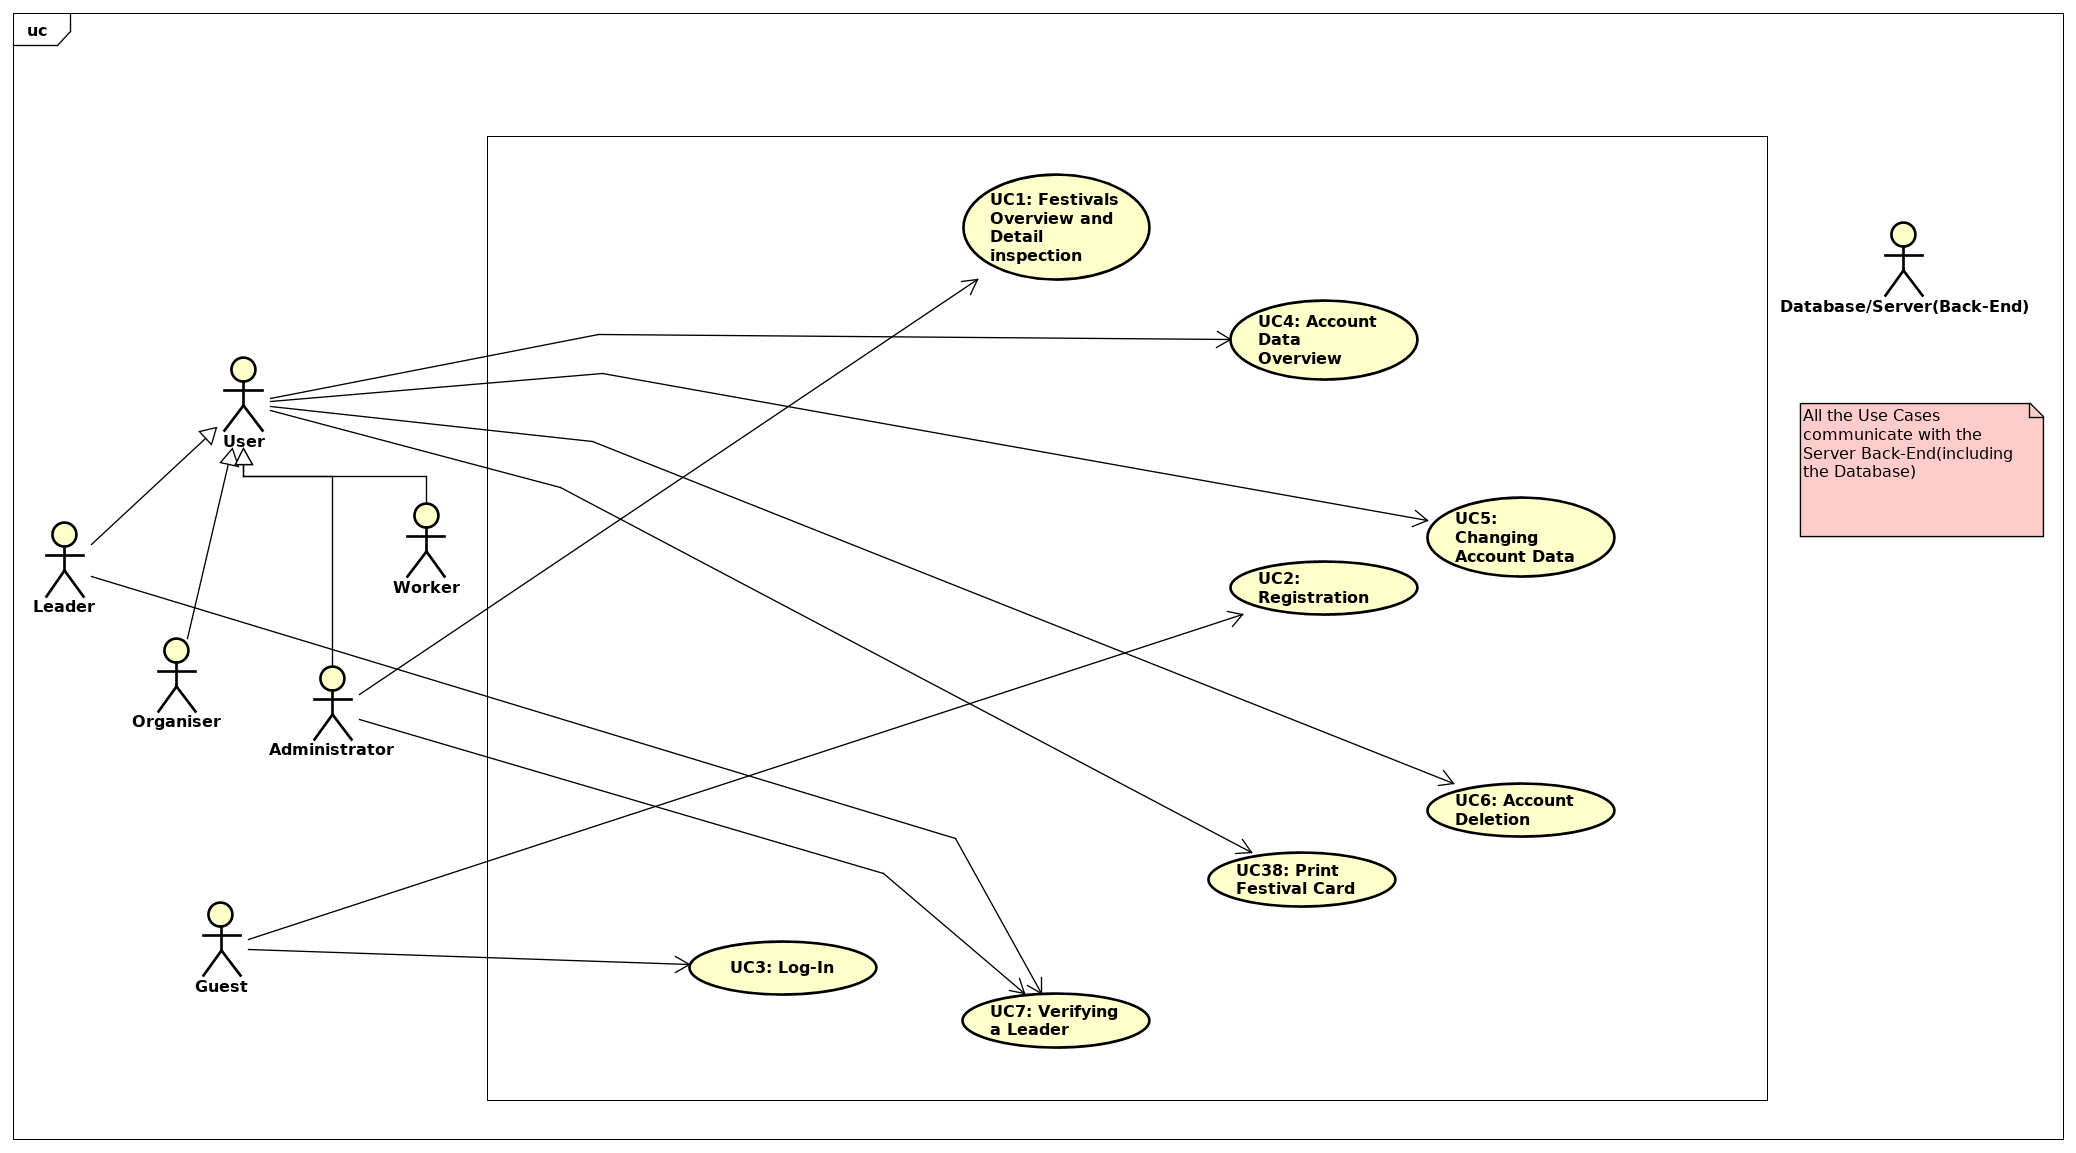
\includegraphics[width=\linewidth]{diagrams/uc-diag0-general.png}
					\caption{Use Case diagram - General Account Usage}
					\label{fig:uc_diag_0_general}
				\end{figure}
			
				\begin{figure}[H]
					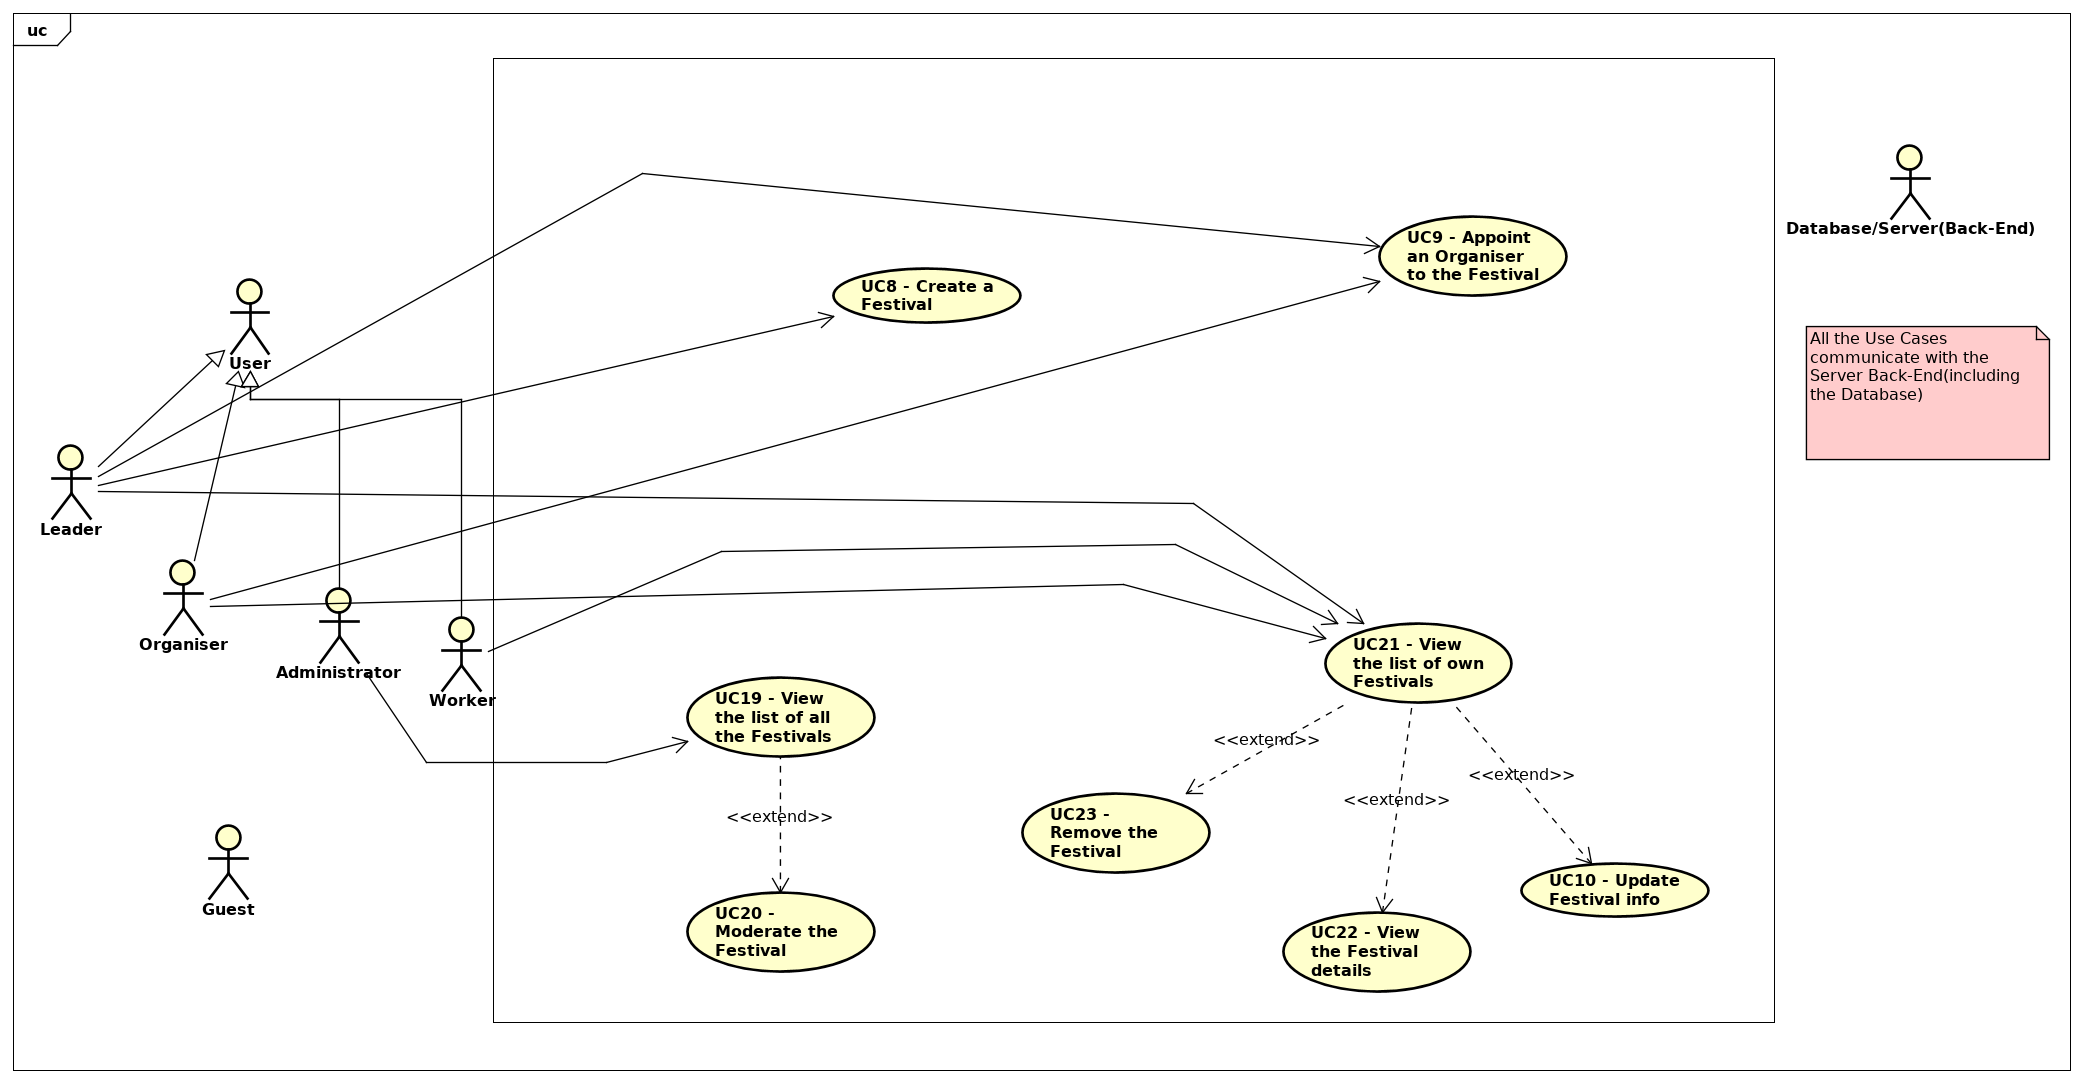
\includegraphics[width=\linewidth]{diagrams/uc-diag1-festival.png}
					\caption{Use Case diagram - Festival}
					\label{fig:uc_diag_1_festival}
				\end{figure}
		
				\begin{figure}[H]
					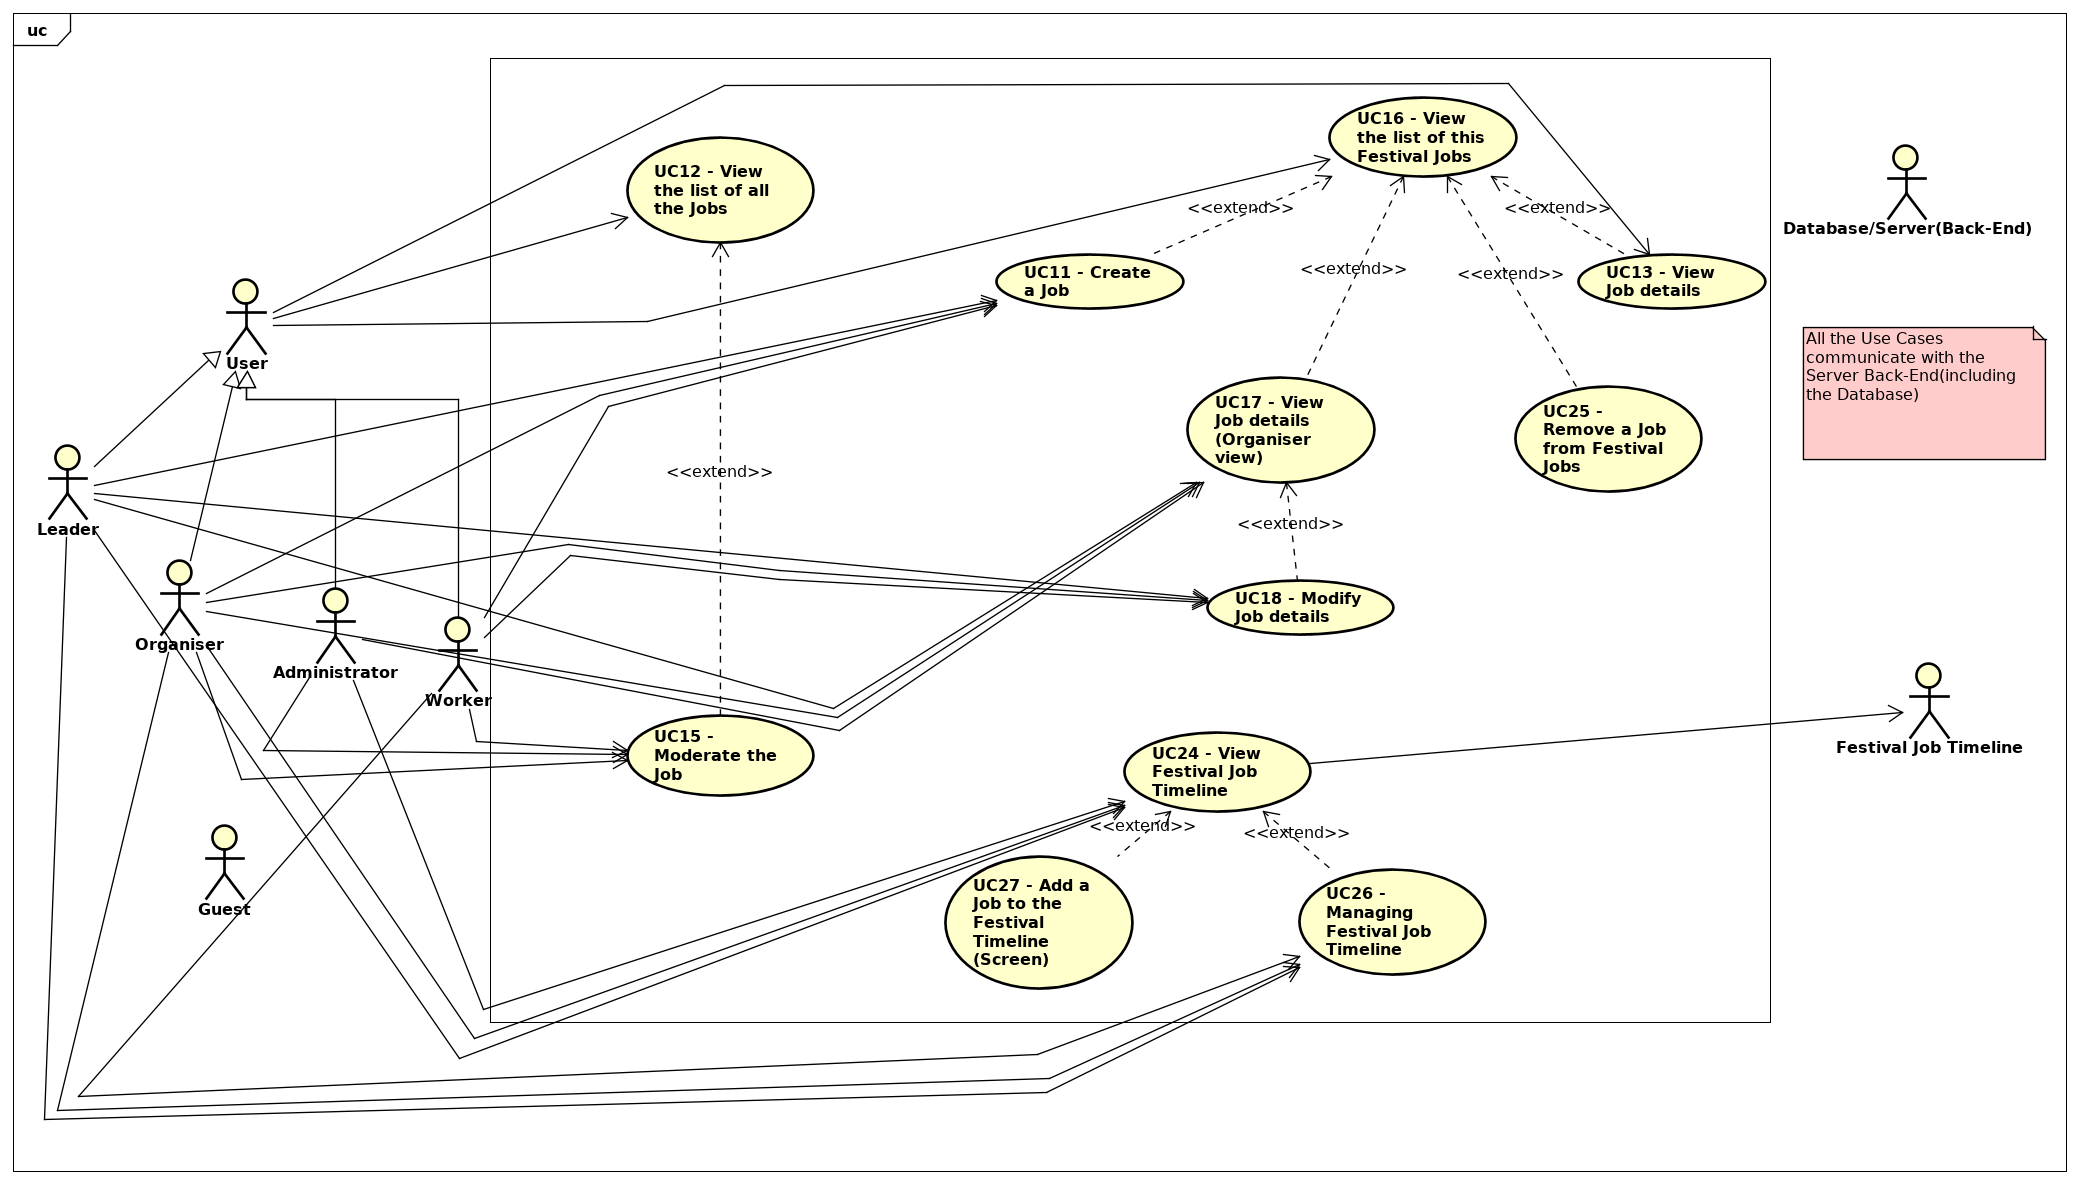
\includegraphics[width=\linewidth]{diagrams/uc-diag2-job.png}
					\caption{Use Case diagram - Job}
					\label{fig:uc_diag_2_job}
				\end{figure}
	
	
				\begin{figure}[H]
					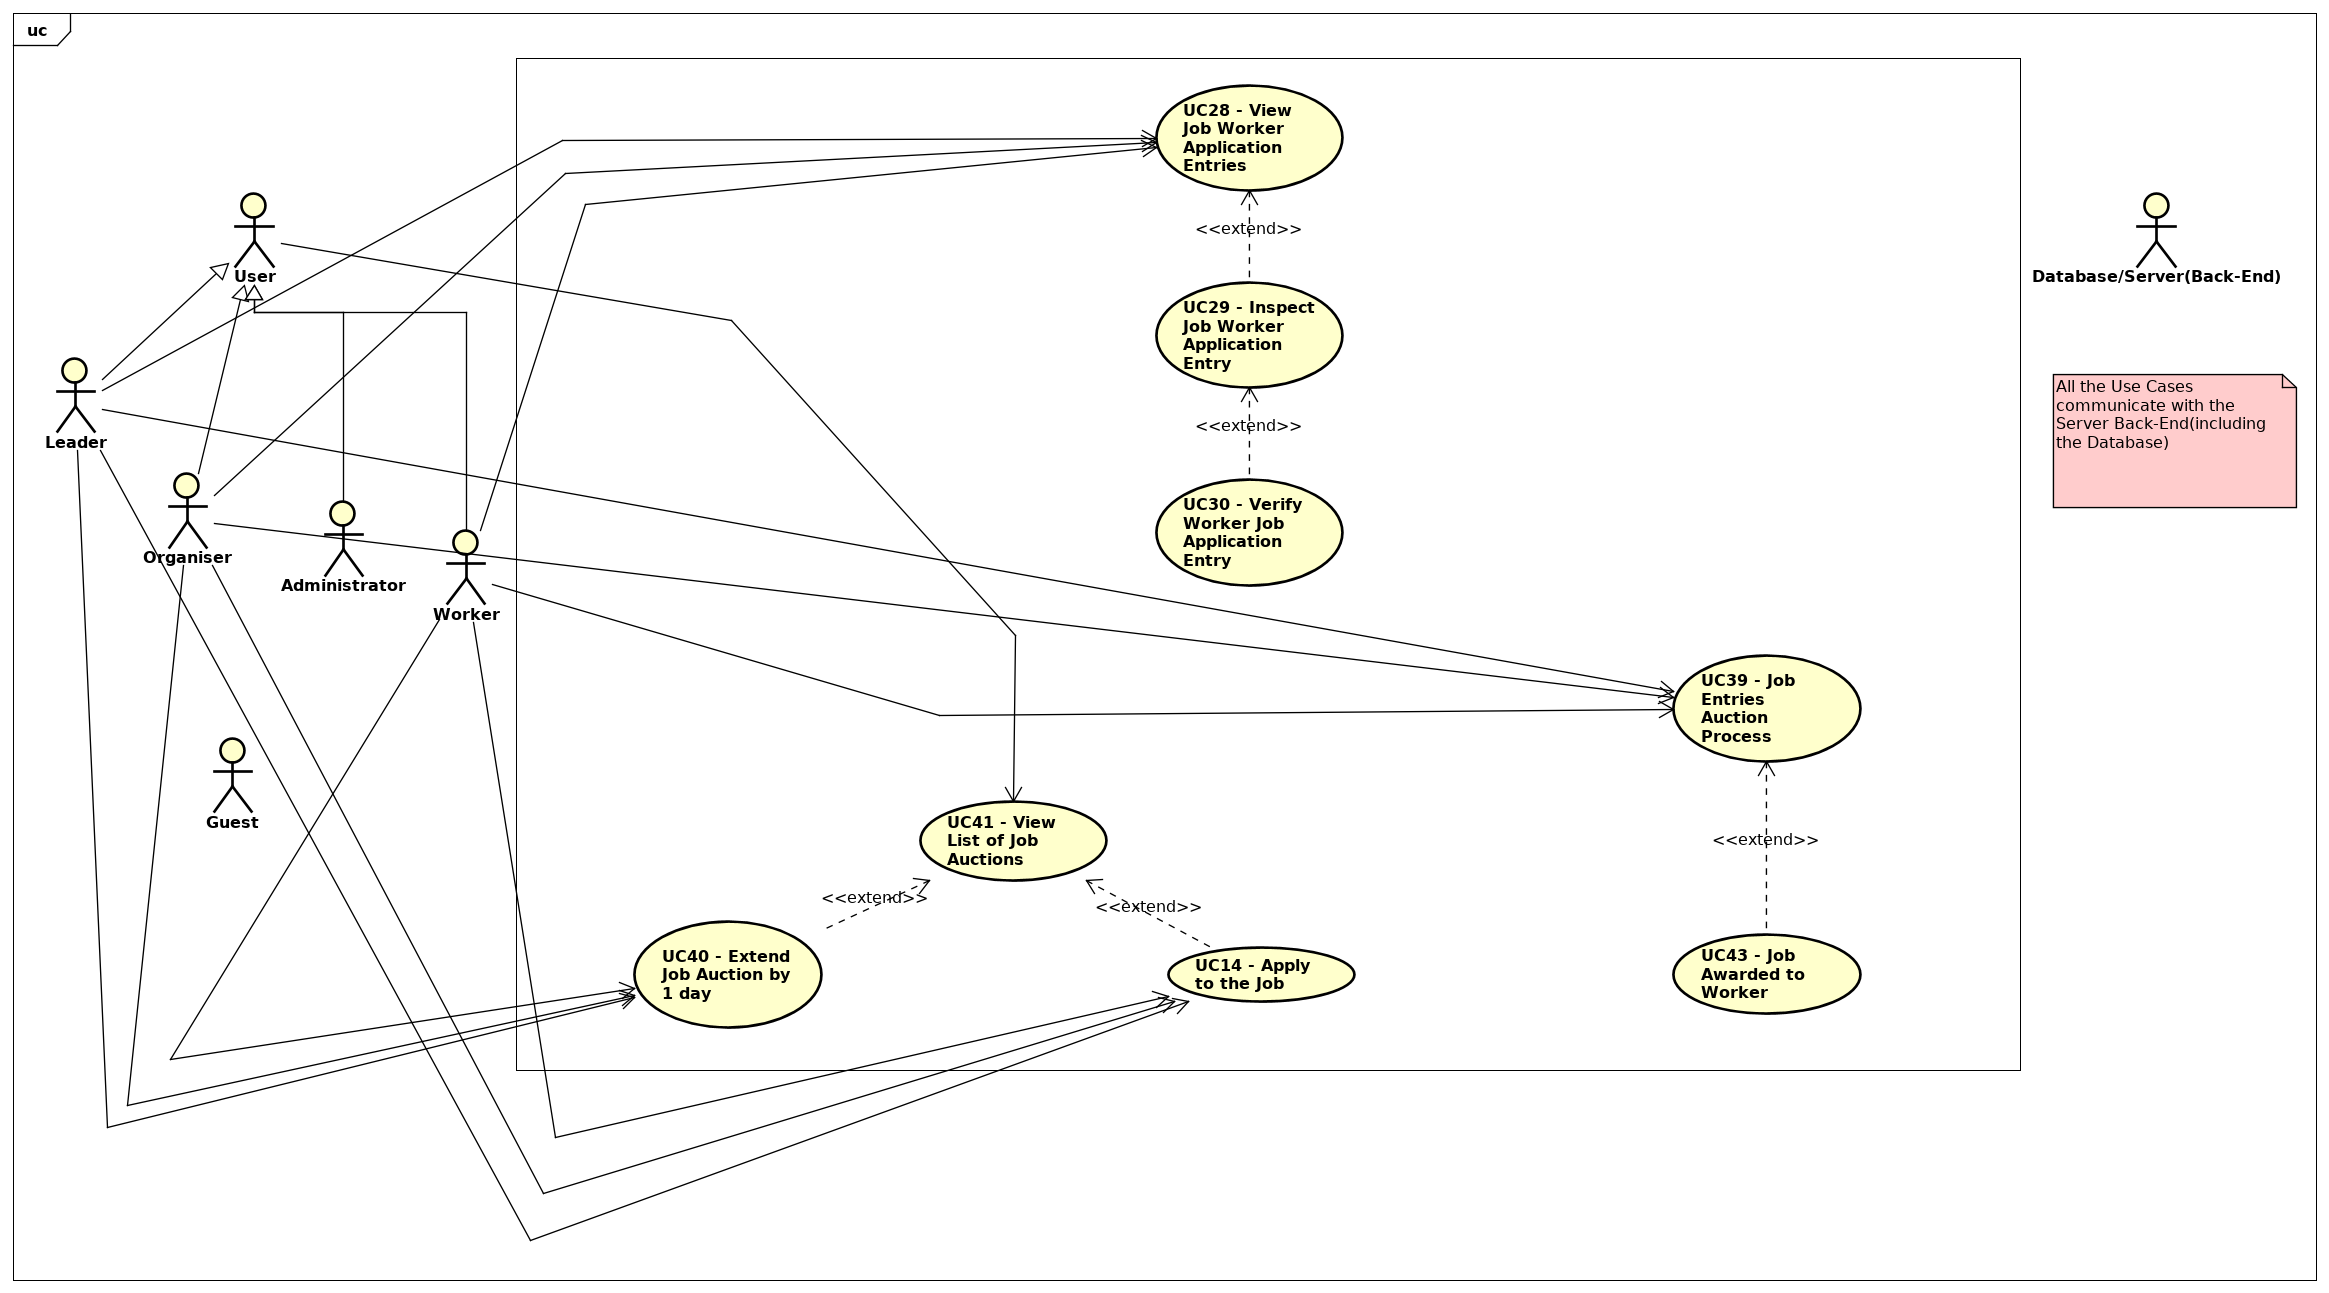
\includegraphics[width=\linewidth]{diagrams/uc-diag3-auction.png}
					\caption{Use Case diagram - Auction}
					\label{fig:uc_diag_3_auction}
				\end{figure}
			
				\begin{figure}[H]
					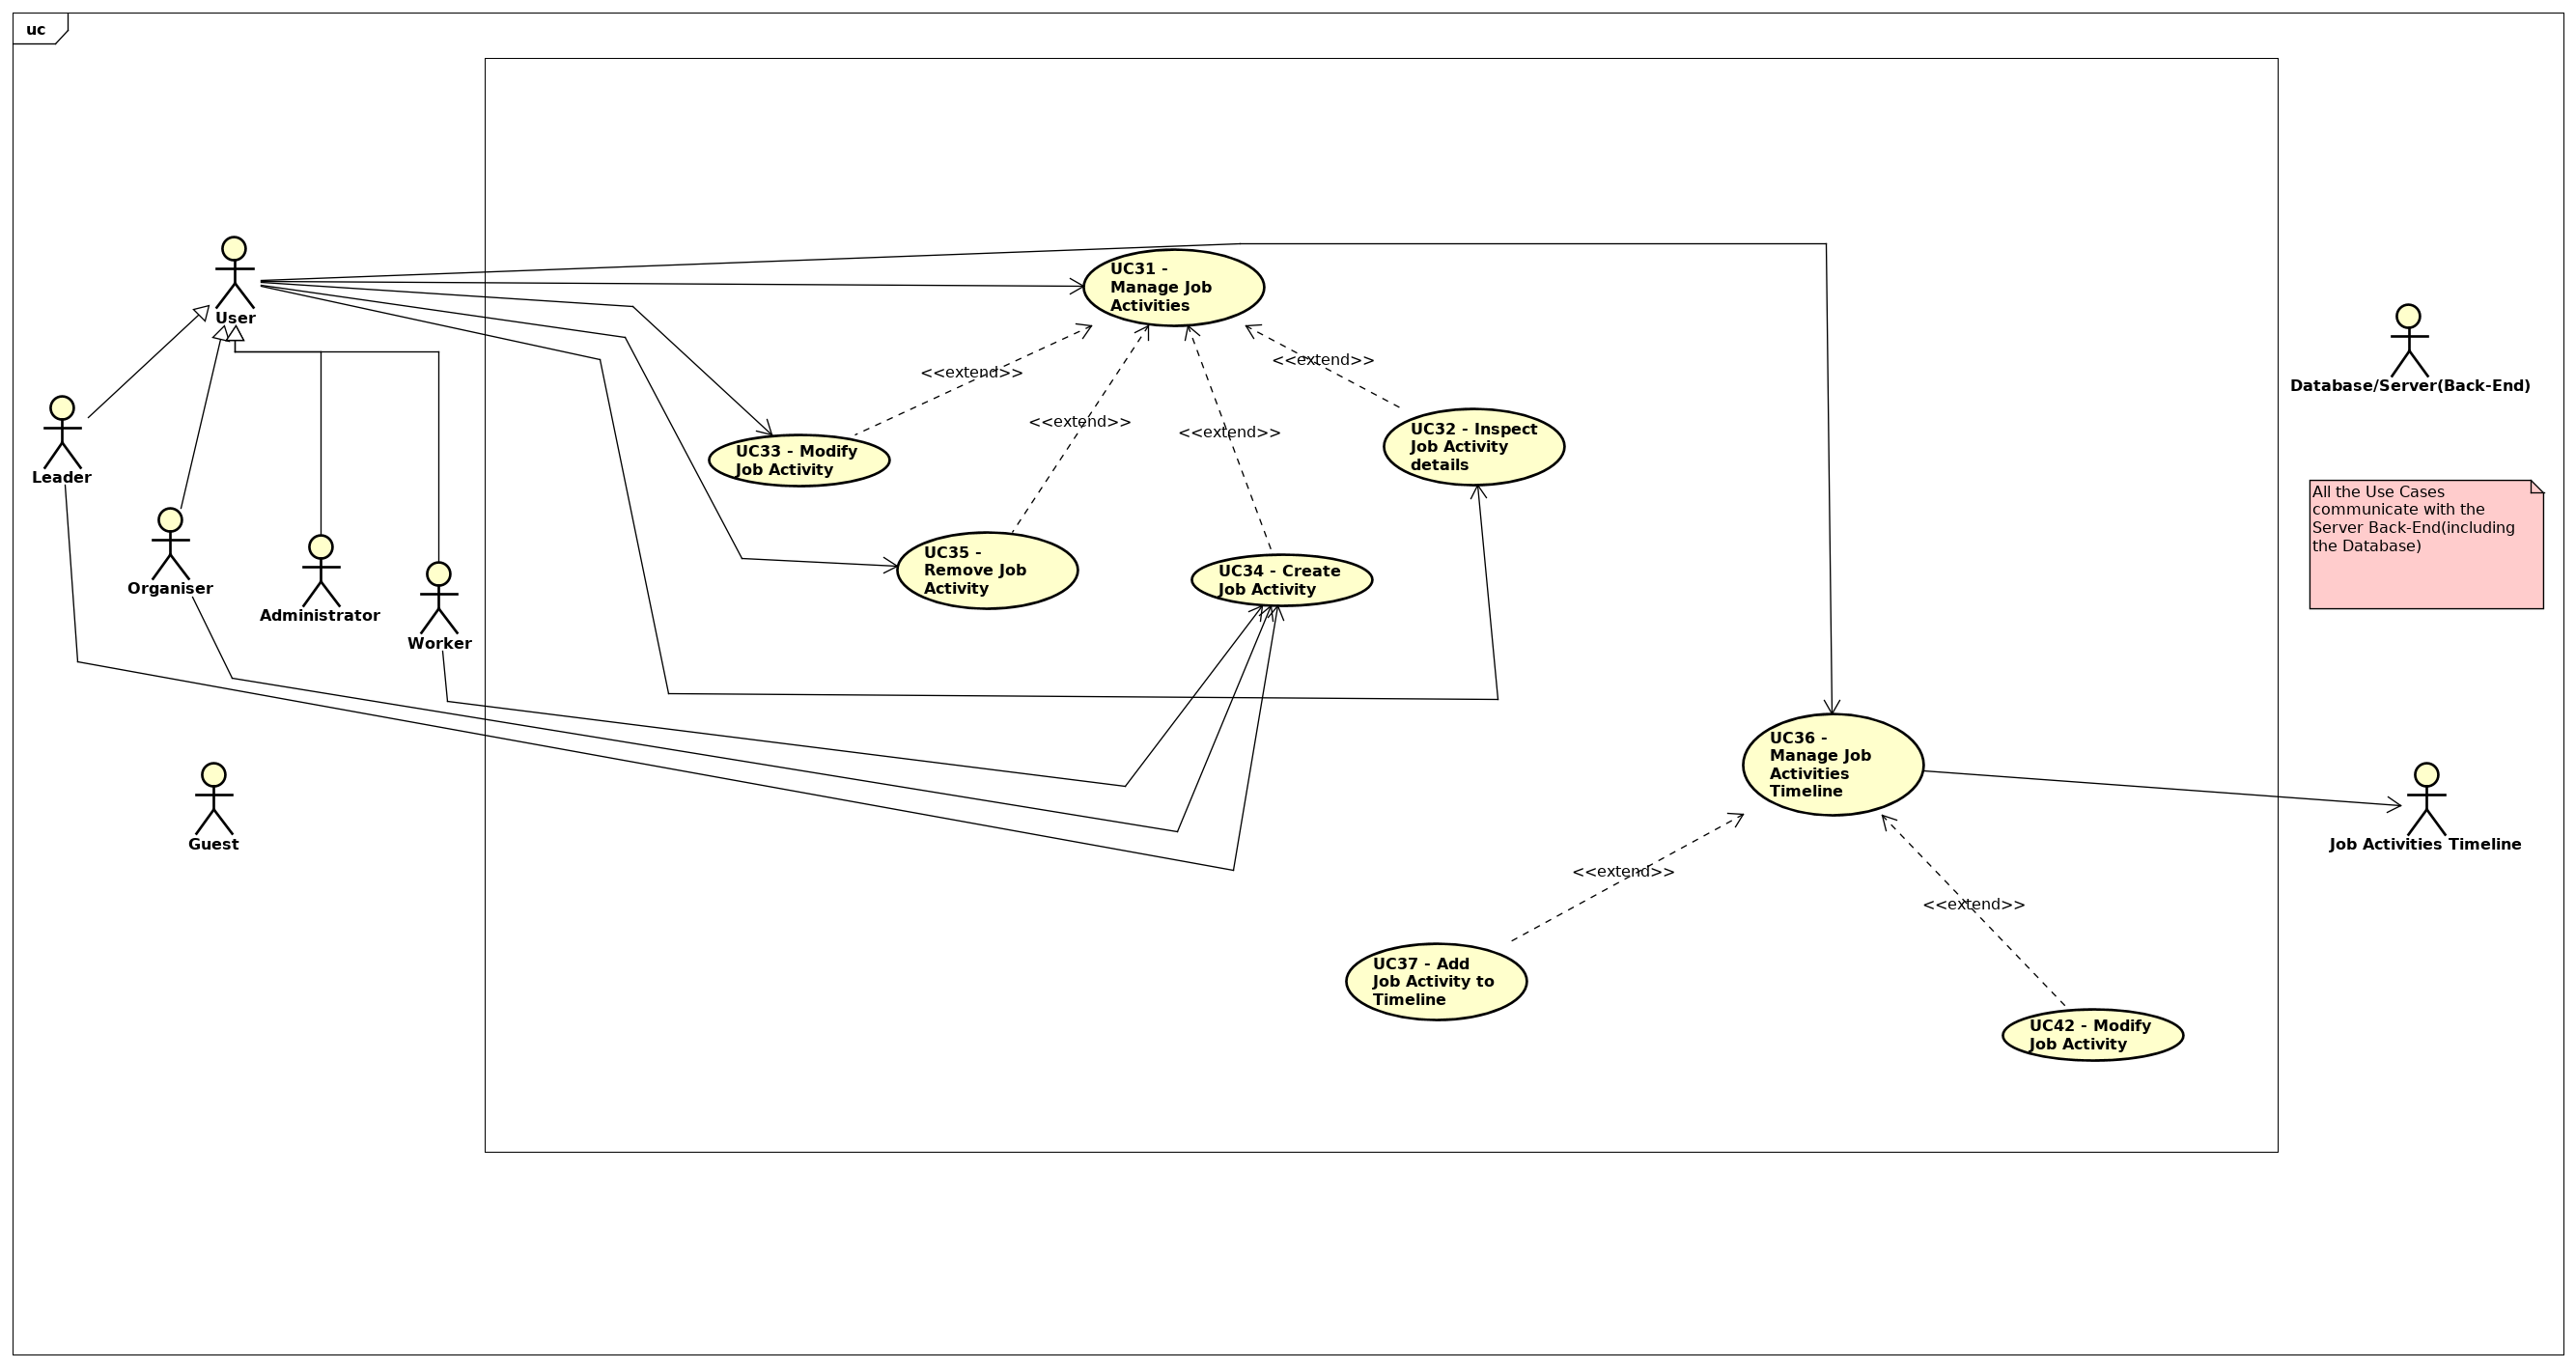
\includegraphics[width=\linewidth]{diagrams/uc-diag4-activity.png}
					\caption{Use Case diagram - Activity}
					\label{fig:uc_diag_4_activity}
				\end{figure}
			
			\eject

			\subsection{Sequence Diagrams}
								
				\textbf{Use Case 31 Manage Job Activities(Worker view)}
				The Worker needs to organise the Job he's been assigned. He does this by creating, modifying and removing(= manipulating) Activities that compose individual Jobs.
				This Use Case depicts the management of such a list of Activities that make up a Job. These Activities can then be added to the Timeline, where their time domain will be well defined and visible - this will enable an easy visualisation of the way the Job will be done and organised.
				\begin{figure}[H]
					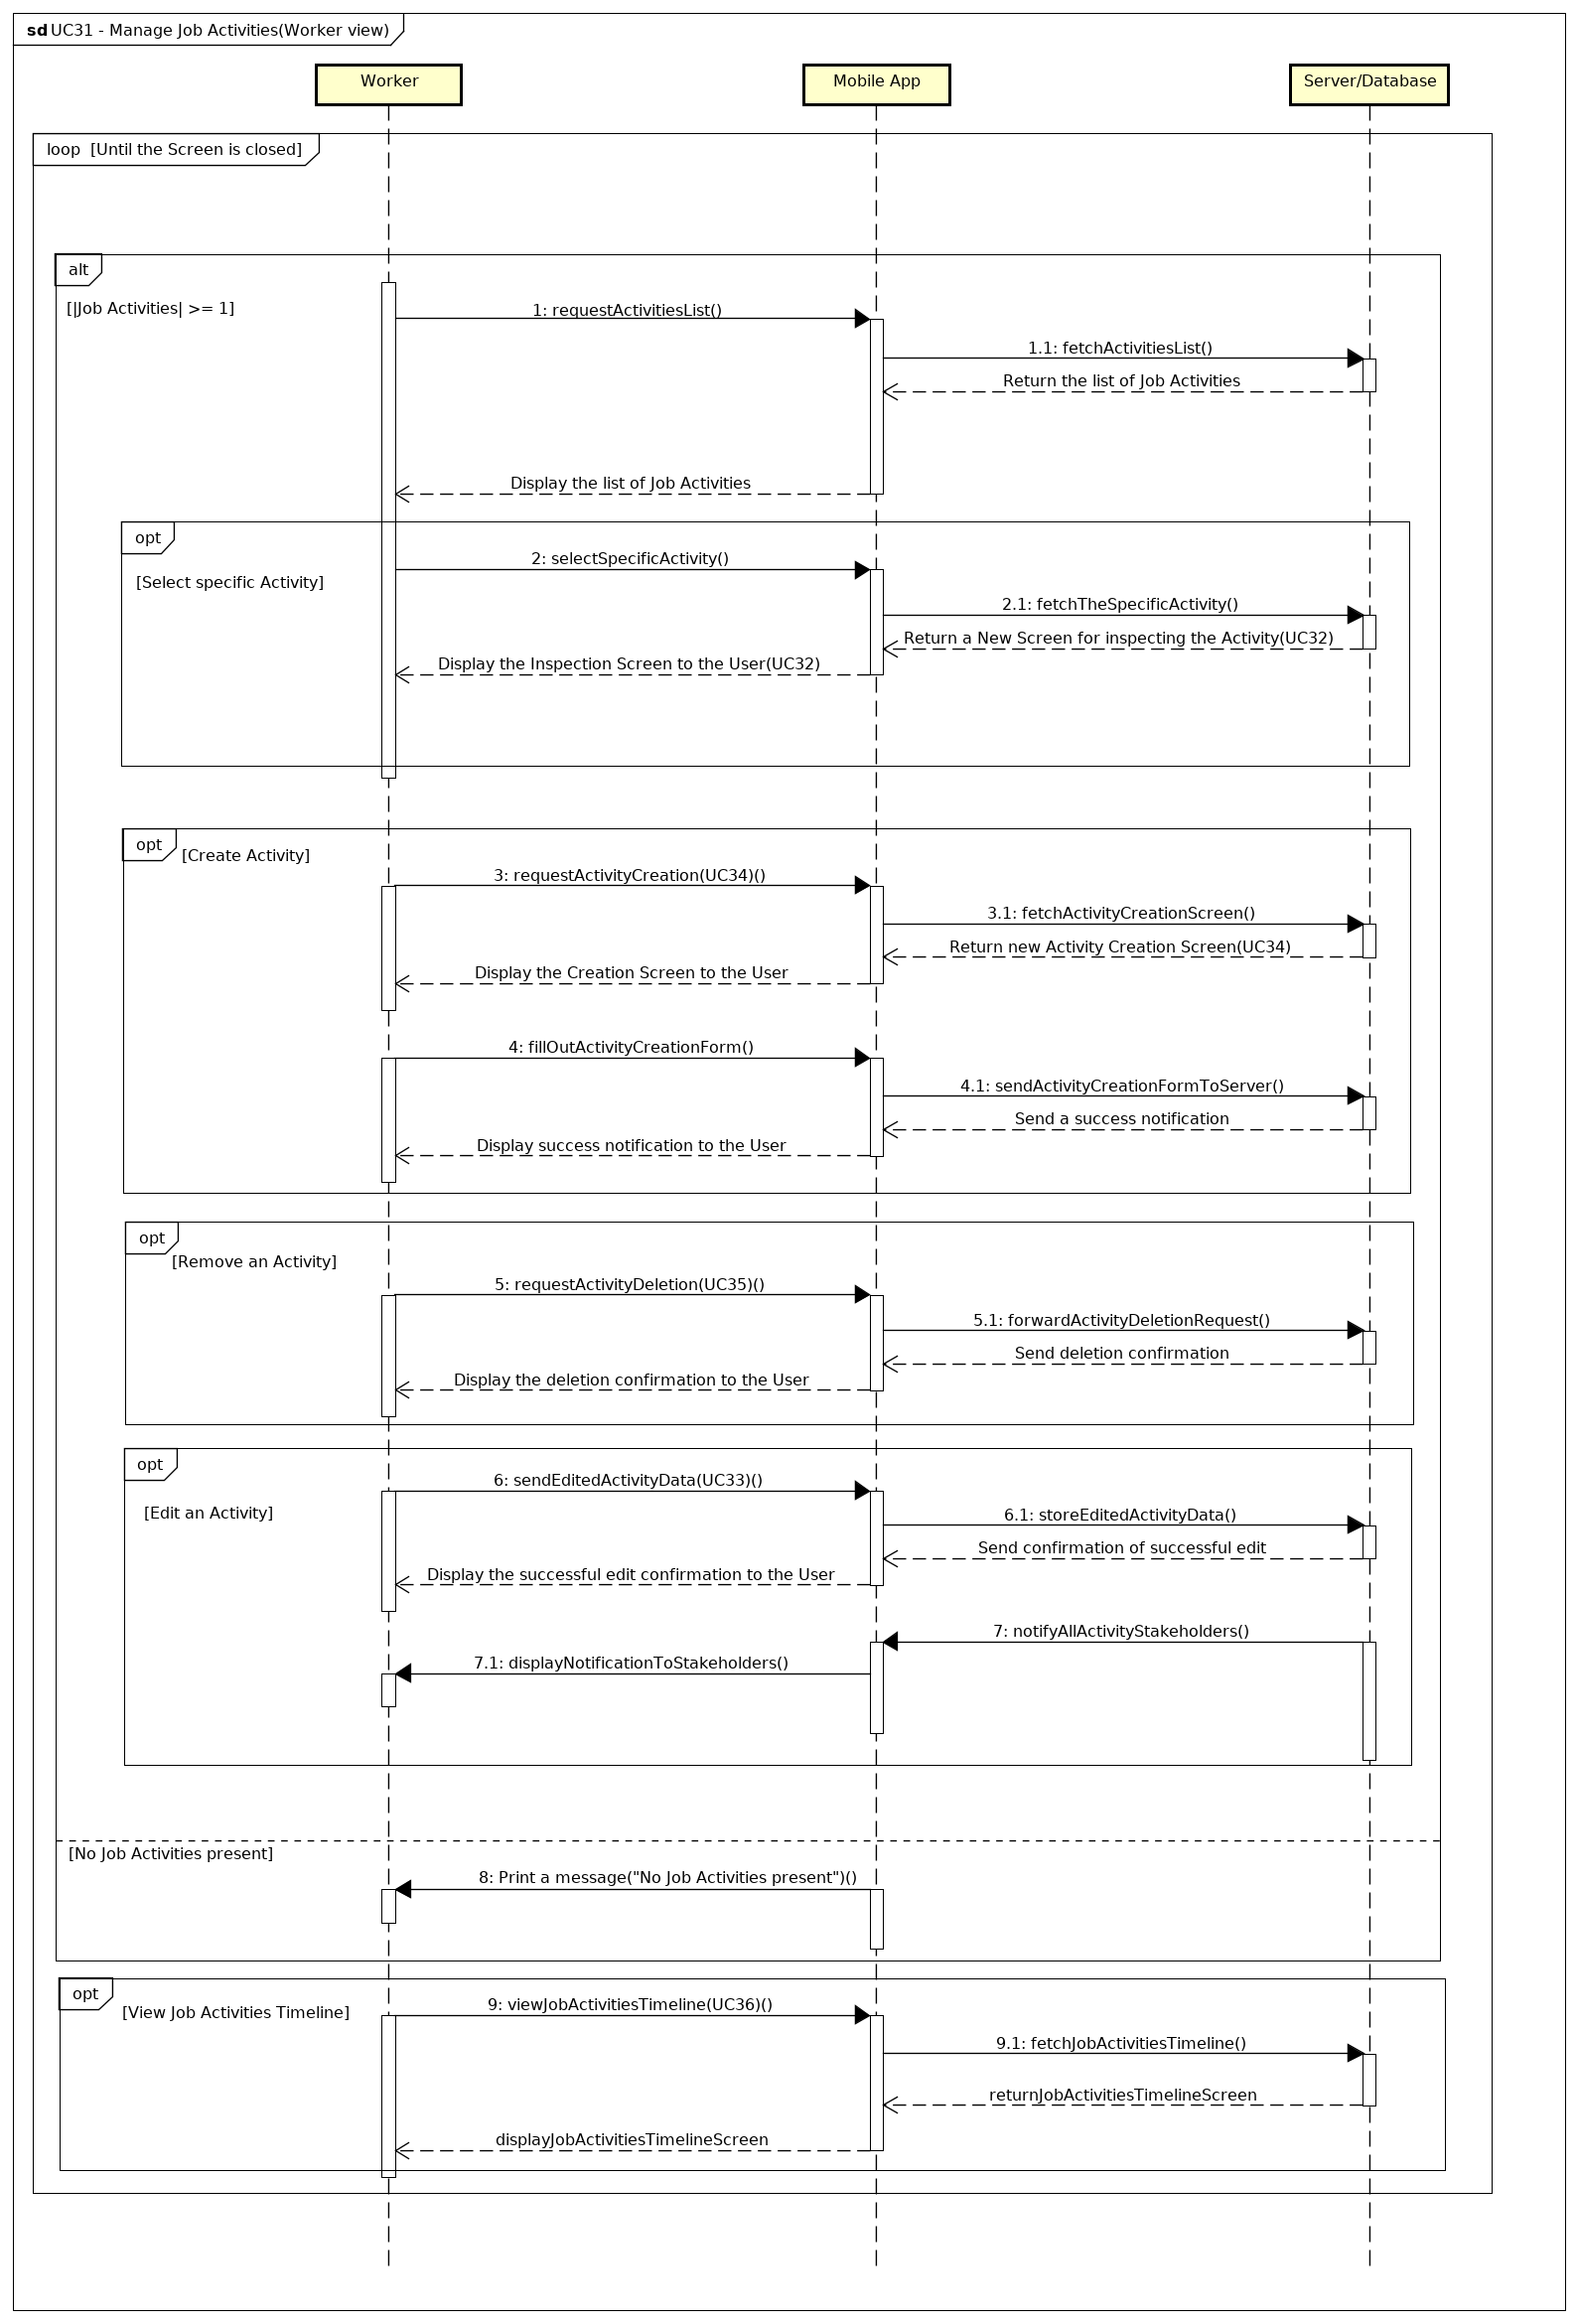
\includegraphics[width=\linewidth]{diagrams/sd-diag0-jobact.png}
					\caption{Job Activities Sequence Diagram}
					\label{fig:sd0_job_activities}
				\end{figure}
				
				\textbf{Use Case 26 Managing Festival Job Timeline}
				It is necessary for the Festival Leader or Organiser to properly manage the Festival Jobs with regard to Time organisation.
				This Use Case allows the Leader/Organiser to define the beginning and end times of certain Job Festivals, as well as modify their durations.
				Timeline is a graphical flowchart - easy and intuitive Festival Job organisation. Concurrency and parallelisation can also be easily achieved.
				
				\begin{figure}[H]
					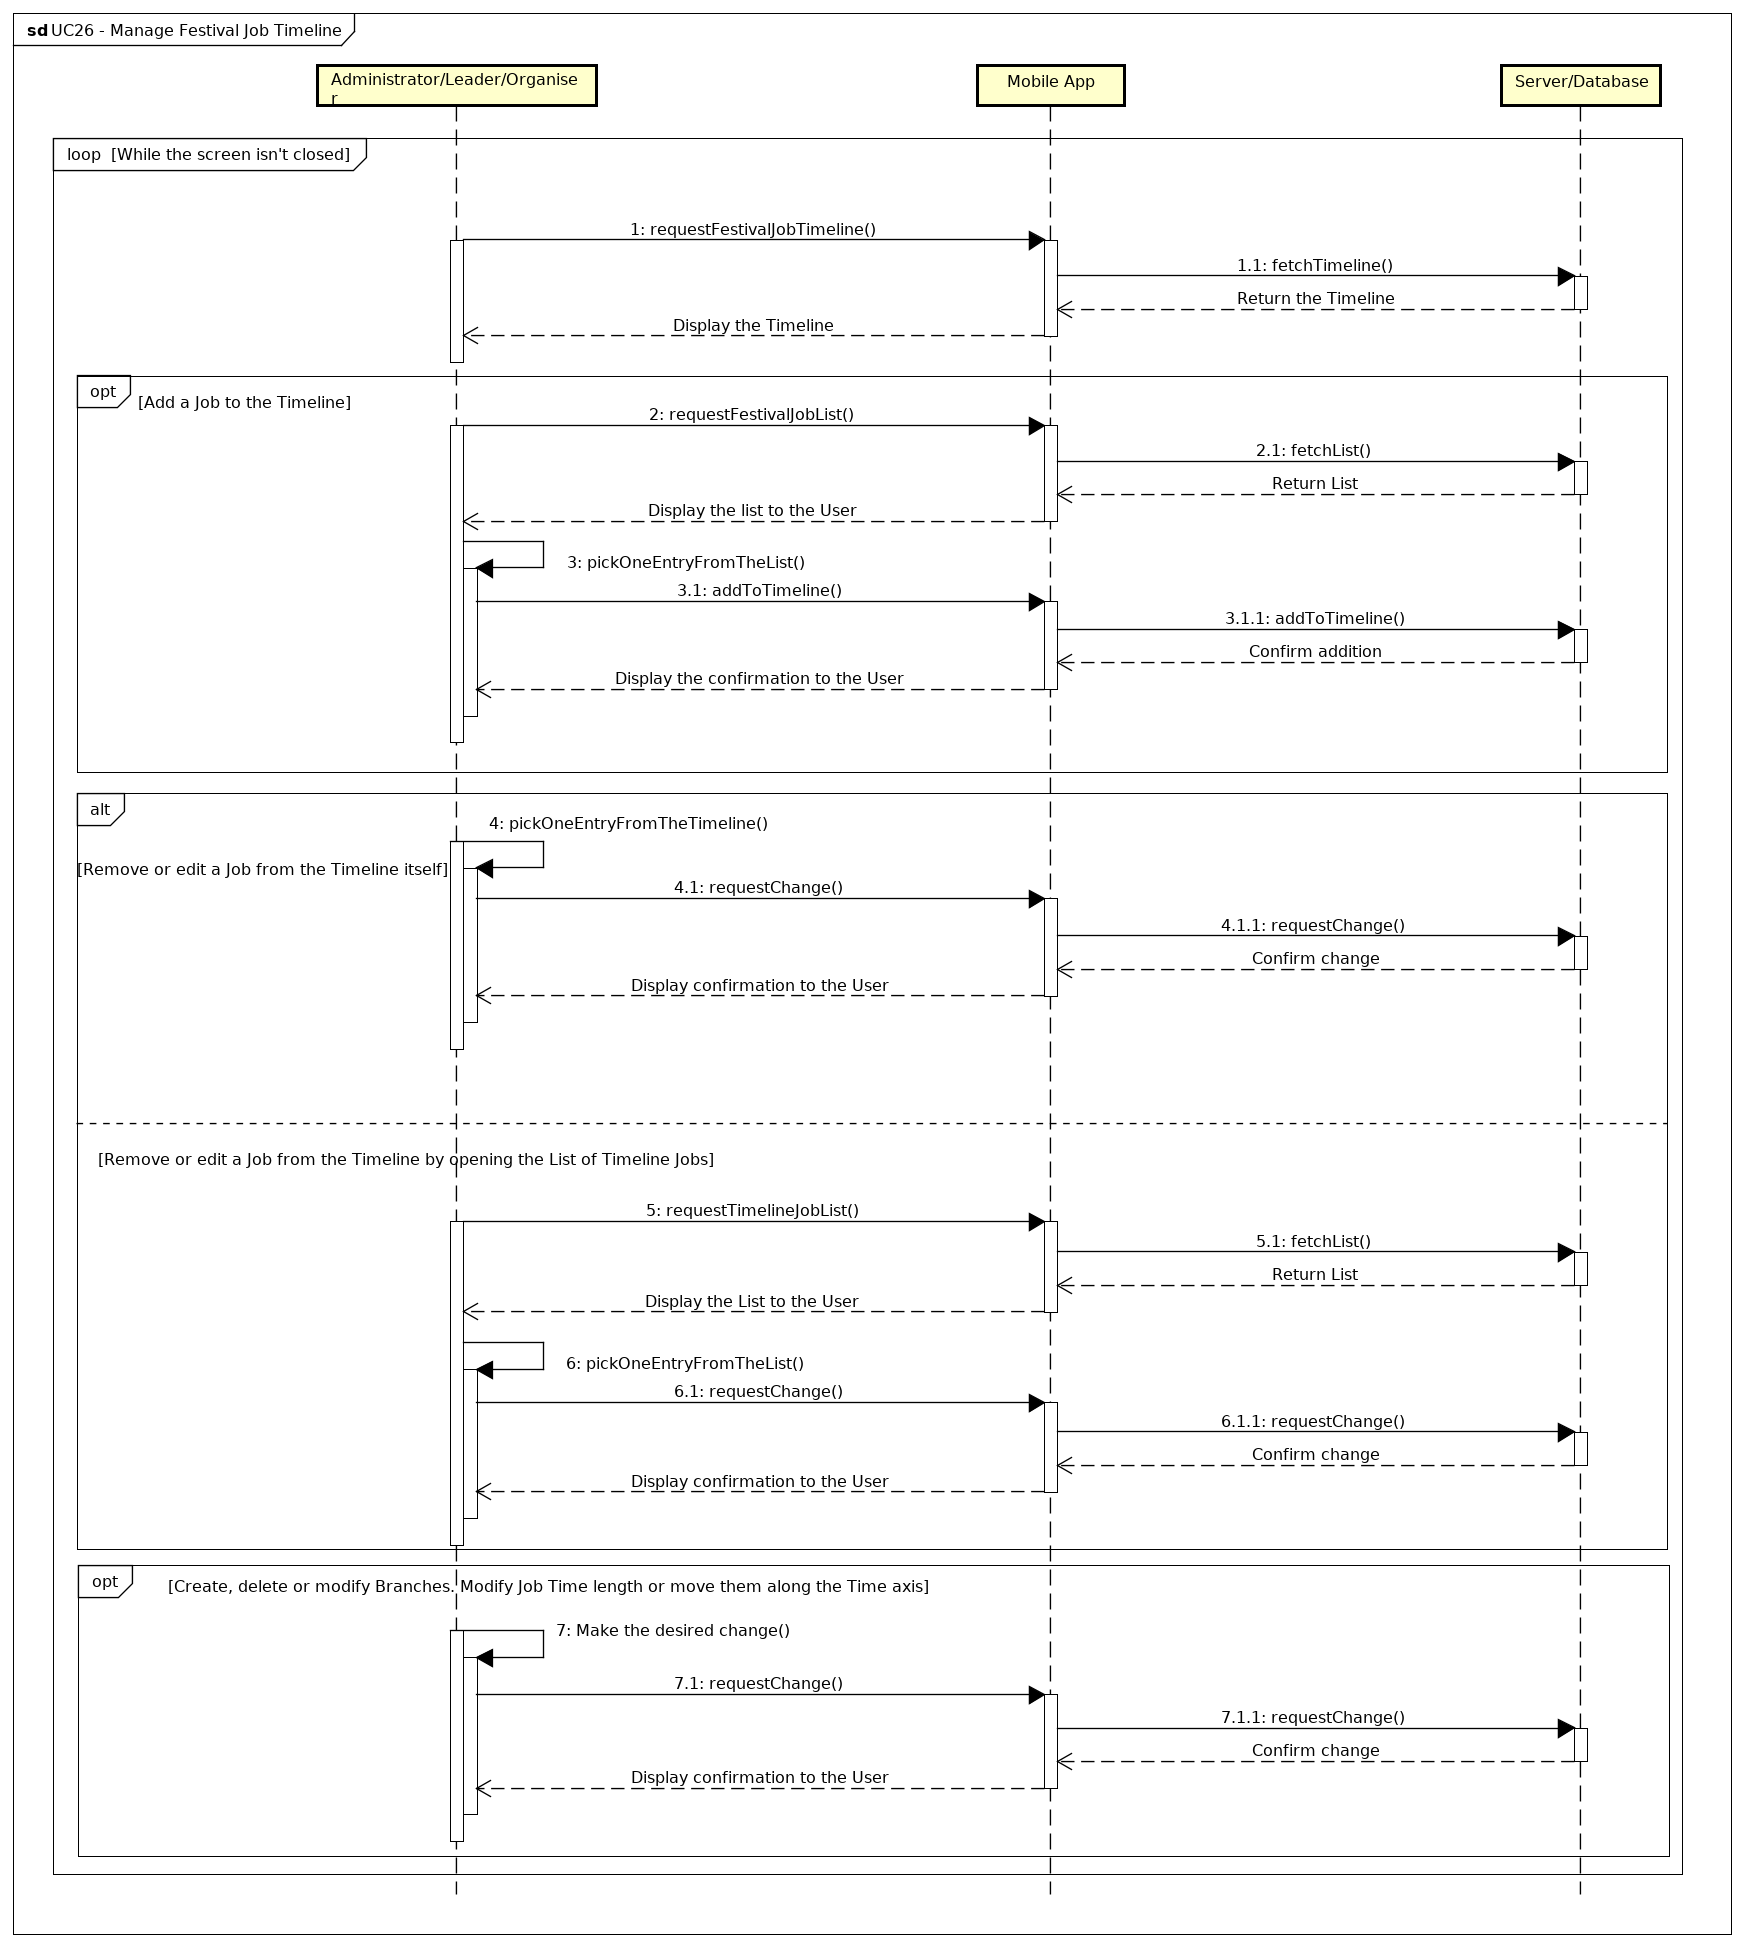
\includegraphics[width=\linewidth]{diagrams/sd-diag1-fjt.png}
					\caption{Festival Job Timeline Sequence Diagram}
					\label{fig:sd1_festival_job_timeline}
				\end{figure}
				
				\textbf{Use Case 36 Manage Job Activities Timeline(Worker view)}
				Just as it is with Festival Leaders and Organiser and Festival Jobs Management so it is with Workers and Job Activities Management.
				Lead Workers must manage their Jobs' Activities in much the same way. They have to take into consideration the start and end times of each Activity, as well as parallelise those Activities.
				The purpose of the Timeline here is, too, to provide an easy, graphical, and intuitive way of doing this Job Activities manipulation and organisation.
				
				\begin{figure}[H]
					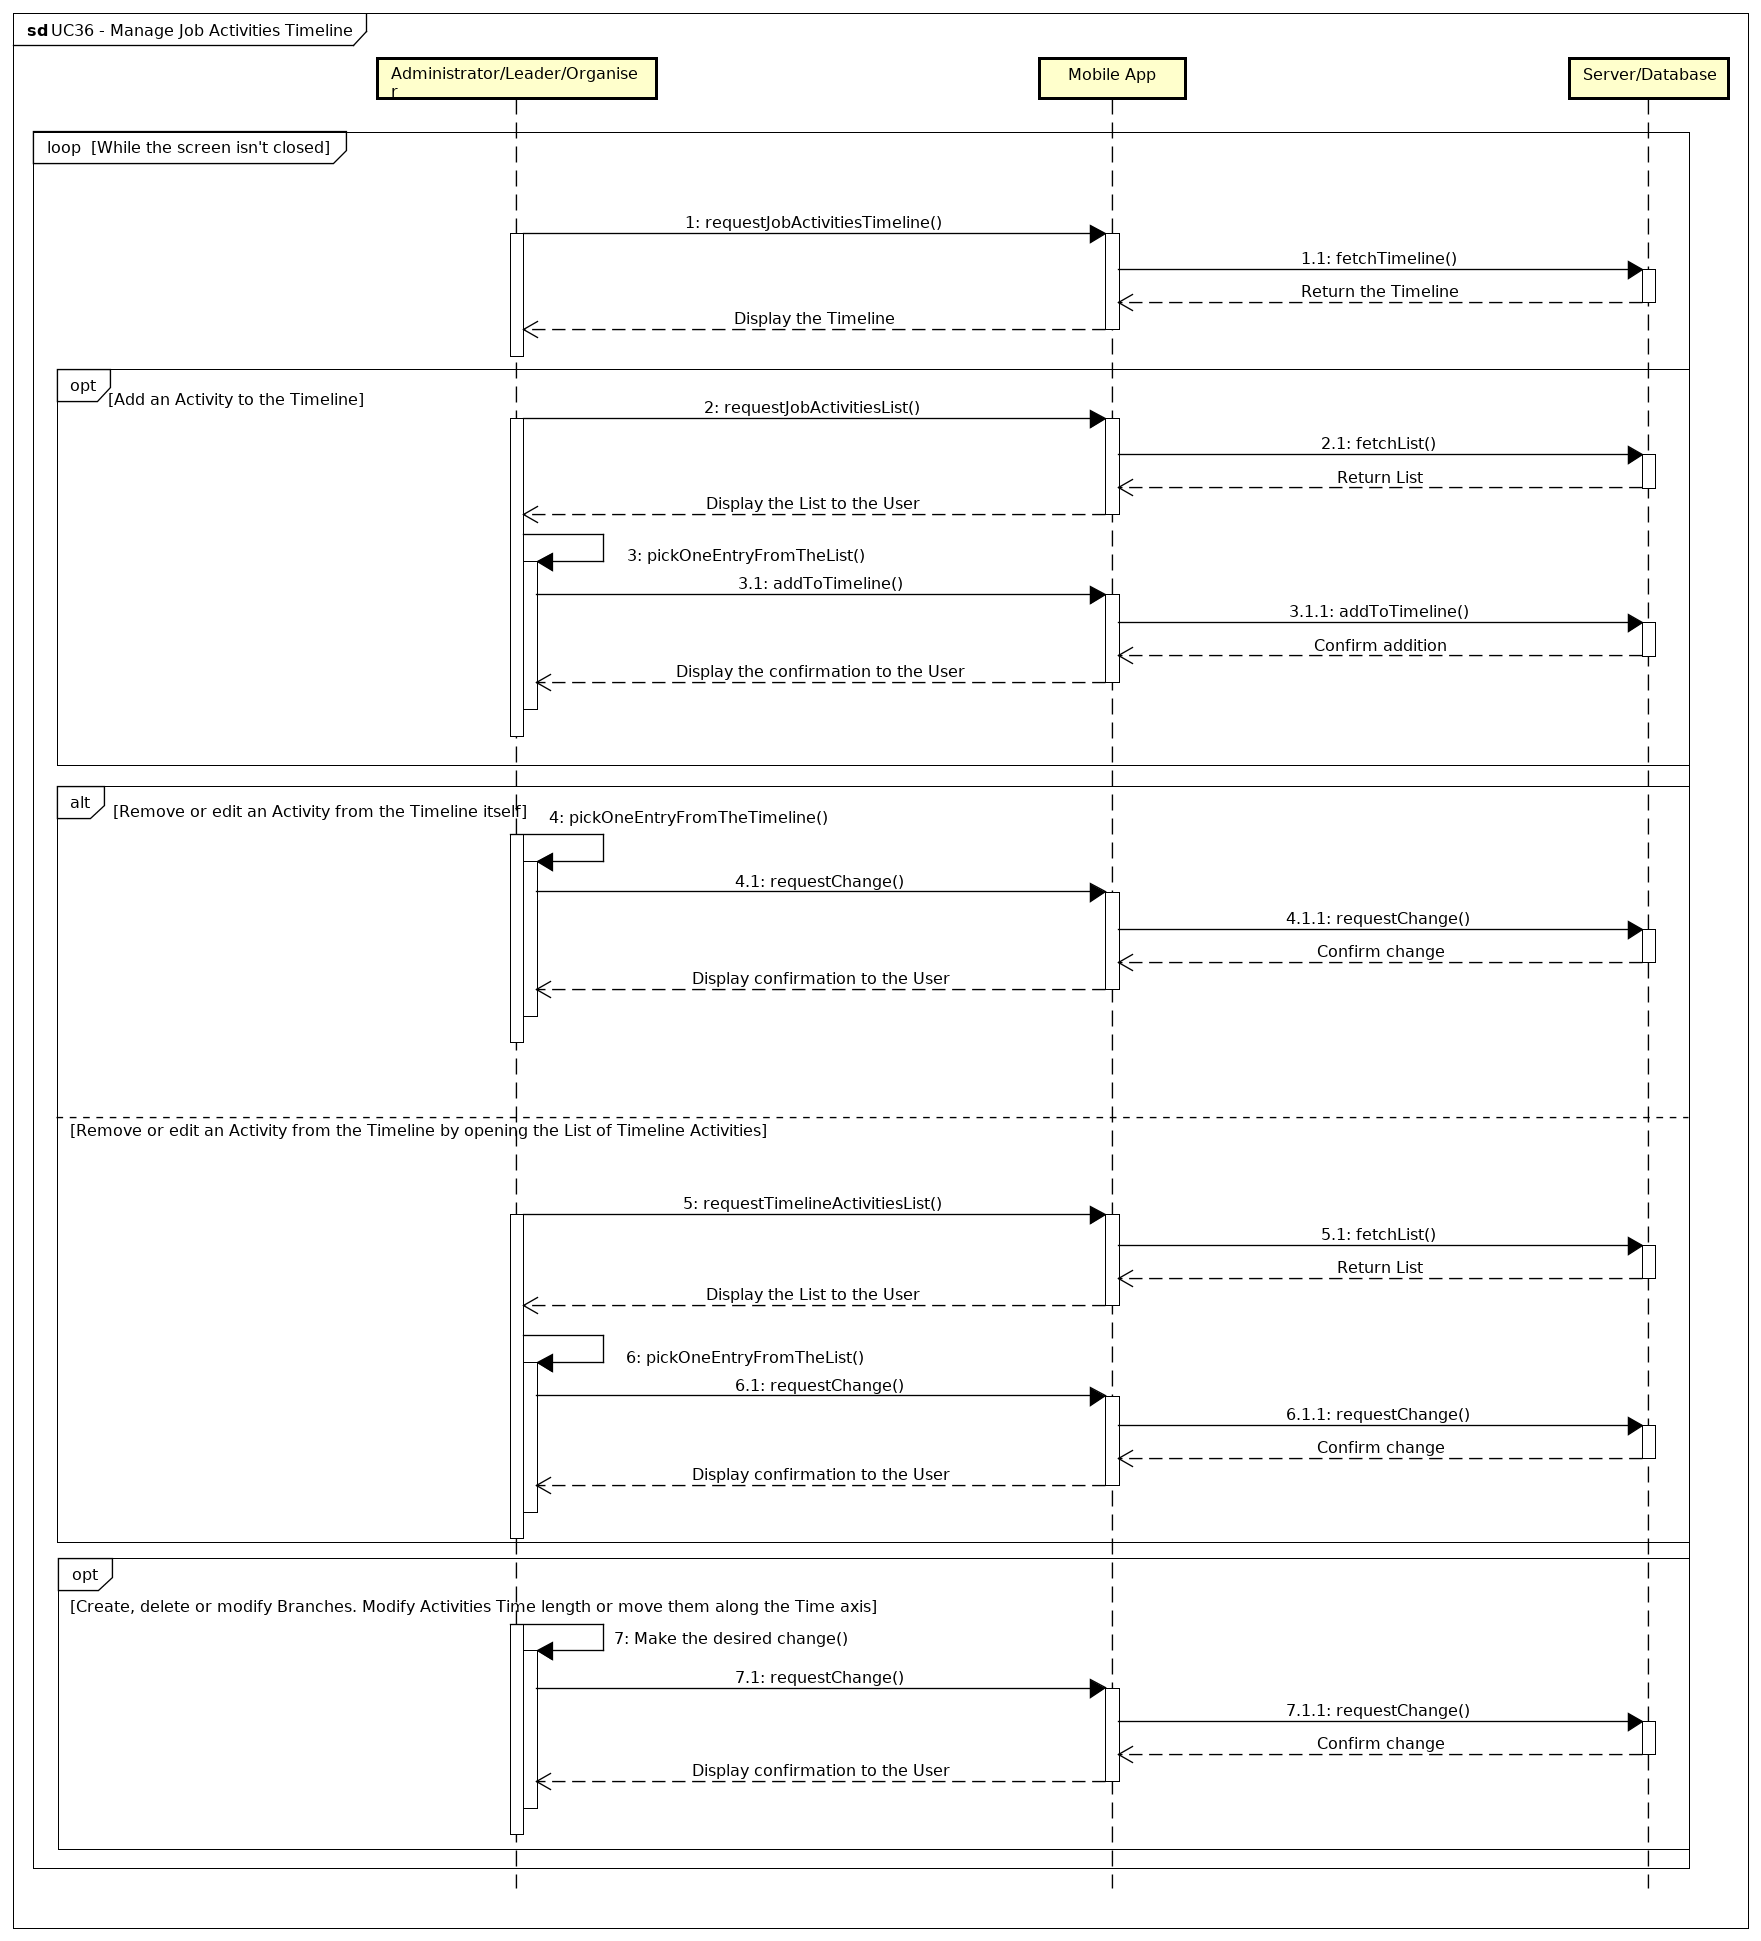
\includegraphics[width=\linewidth]{diagrams/sd-diag2-jat.png}
					\caption{Job Activities Timeline Sequence Diagram}
					\label{fig:sd2_job_activities_timeline}
				\end{figure}
				
				\textbf{Use Case 21 View the List of own Festivals}
				Leaders and Organisers must view the List of the Festivals that they're reponsible for so they can further view the details of those Festivals, and then work on those Festivals.
				This Use Case is one of the pillars of the app, as it enables the management of the selected Festivals - Leaders and Organisers are in charge of those Festivals.

				\begin{figure}[H]
					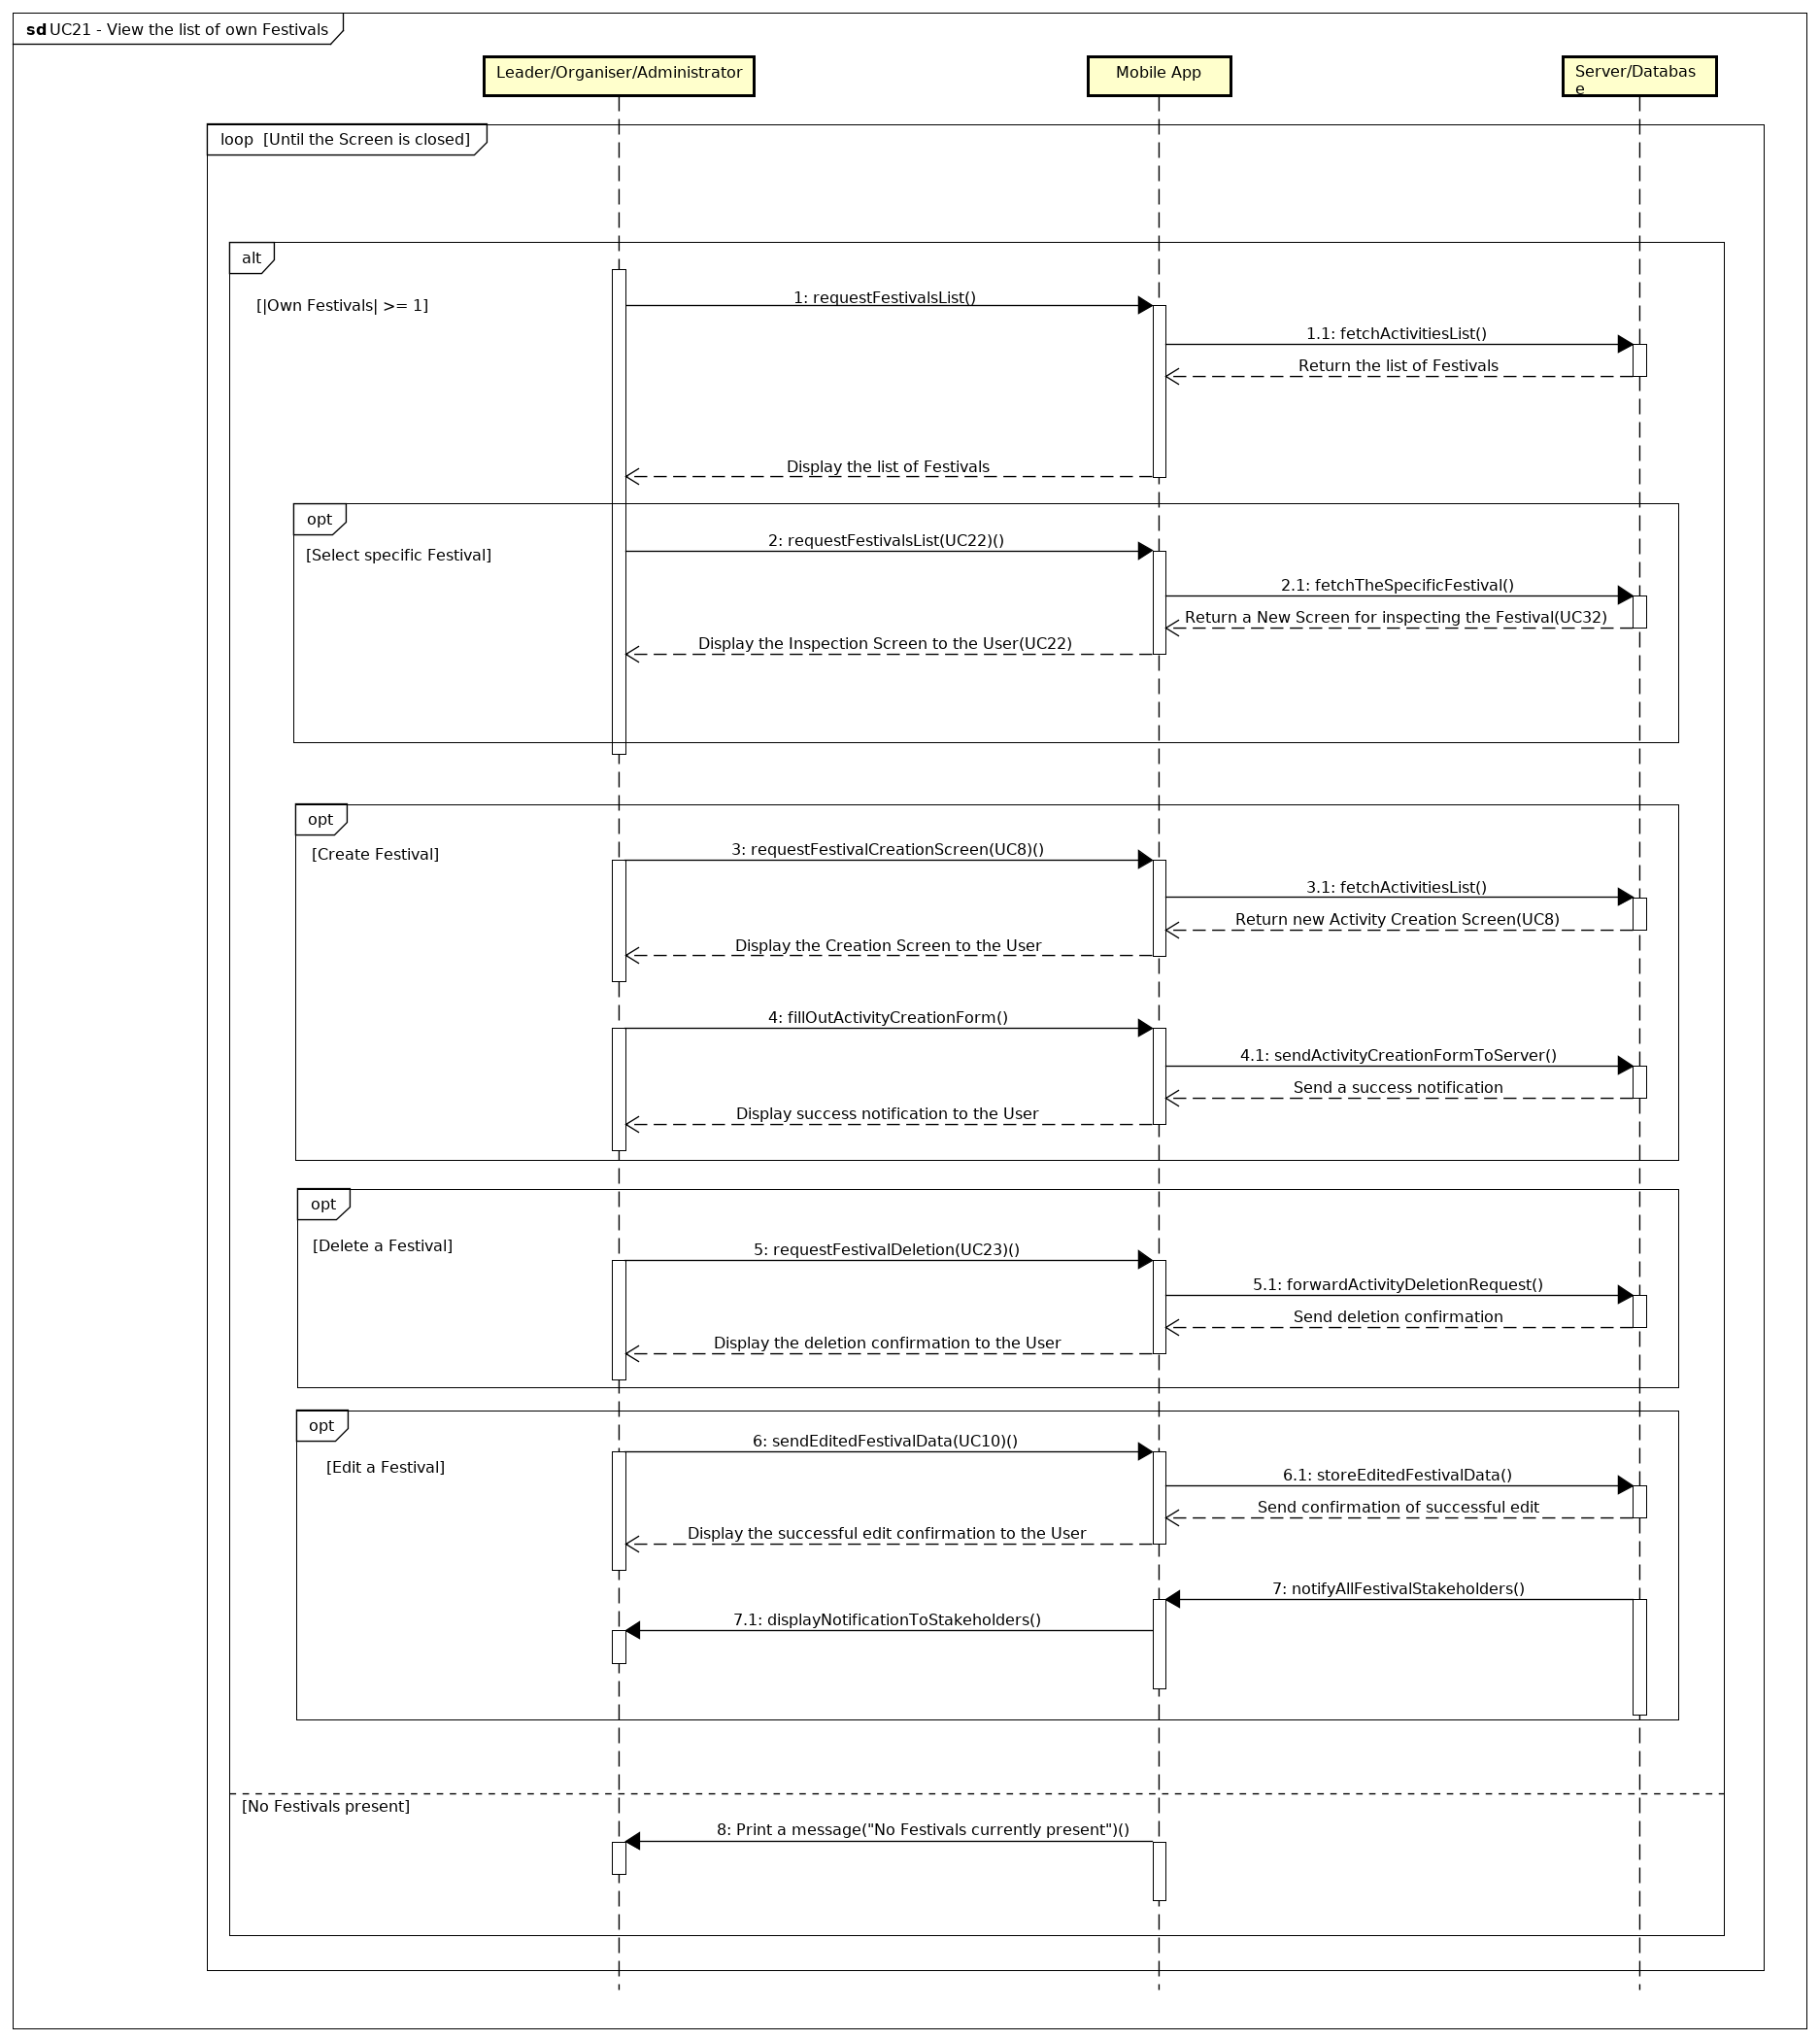
\includegraphics[width=\linewidth]{diagrams/sd-diag3-festivalList.png}
					\caption{Organiser/Leader Festival List Sequence Diagram}
					\label{fig:sd3_festival_list}
				\end{figure}
				
				\eject
	
		\section{Other requirements}
			 
			 \begin{packed_item}
			 	\item The System should allow concurrent usage by multiple Users
			 	\item The System should use UTF-8 - allow diacritical characters
			 	\item The System should use HRK and EUR as currency
			 	\item The System should be fast, reponsive and stable
			 	\item In case of some instability or error, the System should be able to recover gracefully and allow further usage
			 	\item User data should be stored safely and securely, as well as be accordingly encrypted
			 	\item The connection to the Server/Database should be reliable and secure
			 	\item The system should be easy and intuitive to use - not too complicated
			 	\item Implementation - using moder Object-Oriented Programming Languages such as Java or Kotlin
			 	\item The System should be as bug resistant as possible
			 \end{packed_item}